%%%%%%%%%%%%%%%%%%%%%%%%%%%%%%%%%%%%%%%%%
% Masters/Doctoral Thesis
% LaTeX Template
% Version 2.5 (27/8/17)
%
% This template was downloaded from:
% http://www.LaTeXTemplates.com
%
% Version 2.x major modifications by:
% Vel (vel@latextemplates.com)
%
% This template is based on a template by:
% Steve Gunn (http://users.ecs.soton.ac.uk/srg/softwaretools/document/templates/)
% Sunil Patel (http://www.sunilpatel.co.uk/thesis-template/)
%
% Template license:
% CC BY-NC-SA 3.0 (http://creativecommons.org/licenses/by-nc-sa/3.0/)
%
%%%%%%%%%%%%%%%%%%%%%%%%%%%%%%%%%%%%%%%%%

%----------------------------------------------------------------------------------------
%	PACKAGES AND OTHER DOCUMENT CONFIGURATIONS
%----------------------------------------------------------------------------------------

\documentclass[
11pt, % The default document font size, options: 10pt, 11pt, 12pt
oneside, % Two side (alternating margins) for binding by default, uncomment to switch to one side
english, % ngerman for German
singlespacing, % Single line spacing, alternatives: onehalfspacing or doublespacing
%draft, % Uncomment to enable draft mode (no pictures, no links, overfull hboxes indicated)
%nolistspacing, % If the document is onehalfspacing or doublespacing, uncomment this to set spacing in lists to single
%liststotoc, % Uncomment to add the list of figures/tables/etc to the table of contents
%toctotoc, % Uncomment to add the main table of contents to the table of contents
%parskip, % Uncomment to add space between paragraphs
%nohyperref, % Uncomment to not load the hyperref package
headsepline, % Uncomment to get a line under the header
%chapterinoneline, % Uncomment to place the chapter title next to the number on one line
%consistentlayout, % Uncomment to change the layout of the declaration, abstract and acknowledgements pages to match the default layout
]{MastersDoctoralThesis} % The class file specifying the document structure

\usepackage[utf8]{inputenc} % Required for inputting international characters
\usepackage[T1]{fontenc} % Output font encoding for international characters

\usepackage{mathpazo} % Use the Palatino font by default

\usepackage{natbib}
% \usepackage[backend=bibtex,style=authoryear,natbib=true]{biblatex} % Use the bibtex backend with the authoryear citation style (which resembles APA)

% \addbibresource{others.bib} % The filename of the bibliography

\usepackage[autostyle=true]{csquotes} % Required to generate language-dependent quotes in the bibliography

\usepackage{xcolor}
\usepackage[normalem]{ulem}
\usepackage{ifthen}
\usepackage{amssymb}
\usepackage{graphicx}
\usepackage{listings}
\usepackage{amsmath}
\usepackage{minitoc}
\usepackage{float}
\usepackage{array}
\usepackage{hyperref}
\usepackage{nameref}
\usepackage{enumitem}

% Just add % Just add % Just add \input{smalltalkEnv} to your file
% then you can use :
% \begin{lstlisting}[language=Smalltalk]
% false become: true.
% \end{lstlisting}

\usepackage{color}
\usepackage{listings}
\usepackage{etoolbox}

\definecolor{stComment}{rgb}{0.5,0.5,0.5}
\definecolor{stString}{rgb}{0.58,0,0.82}
\definecolor{stKeywords}{rgb}{0.21,0.55,0.7}
\definecolor{stNumbers}{rgb}{.5,0,0}

\newtoggle{InString}{}% Keep track of if we are within a string
\togglefalse{InString}% Assume not initally in string
\newcommand*{\ColorIfNotInString}[1]{\iftoggle{InString}{#1}{\color{stNumbers}#1}}%
\newcommand*{\ProcessQuote}[1]{#1\iftoggle{InString}{\global\togglefalse{InString}}{\global\toggletrue{InString}}}%

\lstdefinelanguage{Smalltalk}{
  keywordstyle=\color{stKeywords},
  commentstyle=\color{stComment},
  stringstyle=\color{stString},
  alsoletter=\#,
  identifierstyle=\idstyle,
  showstringspaces=false,
  morekeywords={true,false,self,super,nil},
  sensitive=true,
  morecomment=[s]{"}{"},
  morestring=[d]',
  style=SmalltalkStyle,
  tabsize=2,
}


\makeatletter%
\newcommand*\idstyle[1]{%
  \expandafter\id@style\the\lst@token{#1}\relax%
}
\def\id@style#1#2\relax{%
  \ifnum\pdfstrcmp{#1}{\#}=0%
  \ttfamily\color{stString} \the\lst@token%
  \else%
  \edef\tempa{\uccode`#1}%
  \edef\tempb{`#1}%
  \ifnum\tempa=\tempb%
  \ttfamily\color{blue} \the\lst@token%
  \else%
  \the\lst@token%
  \fi%
  \fi%
}

\lstdefinestyle{SmalltalkStyle}{
  literate=%
  {^}{{$\uparrow$}}1%
  % {"}{{{\ProcessQuote{"}}}}1% Disable coloring within double quotes
  % {'}{{{\ProcessQuote{'}}}}1% Disable coloring within single quote
  {0}{{{\ColorIfNotInString{0}}}}1%
  {1}{{{\ColorIfNotInString{1}}}}1%
  {2}{{{\ColorIfNotInString{2}}}}1%
  {3}{{{\ColorIfNotInString{3}}}}1%
  {4}{{{\ColorIfNotInString{4}}}}1%
  {5}{{{\ColorIfNotInString{5}}}}1%
  {6}{{{\ColorIfNotInString{6}}}}1%
  {7}{{{\ColorIfNotInString{7}}}}1%
  {8}{{{\ColorIfNotInString{8}}}}1%
  {9}{{{\ColorIfNotInString{9}}}}1%
}
 to your file
% then you can use :
% \begin{lstlisting}[language=Smalltalk]
% false become: true.
% \end{lstlisting}

\usepackage{color}
\usepackage{listings}
\usepackage{etoolbox}

\definecolor{stComment}{rgb}{0.5,0.5,0.5}
\definecolor{stString}{rgb}{0.58,0,0.82}
\definecolor{stKeywords}{rgb}{0.21,0.55,0.7}
\definecolor{stNumbers}{rgb}{.5,0,0}

\newtoggle{InString}{}% Keep track of if we are within a string
\togglefalse{InString}% Assume not initally in string
\newcommand*{\ColorIfNotInString}[1]{\iftoggle{InString}{#1}{\color{stNumbers}#1}}%
\newcommand*{\ProcessQuote}[1]{#1\iftoggle{InString}{\global\togglefalse{InString}}{\global\toggletrue{InString}}}%

\lstdefinelanguage{Smalltalk}{
  keywordstyle=\color{stKeywords},
  commentstyle=\color{stComment},
  stringstyle=\color{stString},
  alsoletter=\#,
  identifierstyle=\idstyle,
  showstringspaces=false,
  morekeywords={true,false,self,super,nil},
  sensitive=true,
  morecomment=[s]{"}{"},
  morestring=[d]',
  style=SmalltalkStyle,
  tabsize=2,
}


\makeatletter%
\newcommand*\idstyle[1]{%
  \expandafter\id@style\the\lst@token{#1}\relax%
}
\def\id@style#1#2\relax{%
  \ifnum\pdfstrcmp{#1}{\#}=0%
  \ttfamily\color{stString} \the\lst@token%
  \else%
  \edef\tempa{\uccode`#1}%
  \edef\tempb{`#1}%
  \ifnum\tempa=\tempb%
  \ttfamily\color{blue} \the\lst@token%
  \else%
  \the\lst@token%
  \fi%
  \fi%
}

\lstdefinestyle{SmalltalkStyle}{
  literate=%
  {^}{{$\uparrow$}}1%
  % {"}{{{\ProcessQuote{"}}}}1% Disable coloring within double quotes
  % {'}{{{\ProcessQuote{'}}}}1% Disable coloring within single quote
  {0}{{{\ColorIfNotInString{0}}}}1%
  {1}{{{\ColorIfNotInString{1}}}}1%
  {2}{{{\ColorIfNotInString{2}}}}1%
  {3}{{{\ColorIfNotInString{3}}}}1%
  {4}{{{\ColorIfNotInString{4}}}}1%
  {5}{{{\ColorIfNotInString{5}}}}1%
  {6}{{{\ColorIfNotInString{6}}}}1%
  {7}{{{\ColorIfNotInString{7}}}}1%
  {8}{{{\ColorIfNotInString{8}}}}1%
  {9}{{{\ColorIfNotInString{9}}}}1%
}
 to your file
% then you can use :
% \begin{lstlisting}[language=Smalltalk]
% false become: true.
% \end{lstlisting}

\usepackage{color}
\usepackage{listings}
\usepackage{etoolbox}

\definecolor{stComment}{rgb}{0.5,0.5,0.5}
\definecolor{stString}{rgb}{0.58,0,0.82}
\definecolor{stKeywords}{rgb}{0.21,0.55,0.7}
\definecolor{stNumbers}{rgb}{.5,0,0}

\newtoggle{InString}{}% Keep track of if we are within a string
\togglefalse{InString}% Assume not initally in string
\newcommand*{\ColorIfNotInString}[1]{\iftoggle{InString}{#1}{\color{stNumbers}#1}}%
\newcommand*{\ProcessQuote}[1]{#1\iftoggle{InString}{\global\togglefalse{InString}}{\global\toggletrue{InString}}}%

\lstdefinelanguage{Smalltalk}{
  keywordstyle=\color{stKeywords},
  commentstyle=\color{stComment},
  stringstyle=\color{stString},
  alsoletter=\#,
  identifierstyle=\idstyle,
  showstringspaces=false,
  morekeywords={true,false,self,super,nil},
  sensitive=true,
  morecomment=[s]{"}{"},
  morestring=[d]',
  style=SmalltalkStyle,
  tabsize=2,
}


\makeatletter%
\newcommand*\idstyle[1]{%
  \expandafter\id@style\the\lst@token{#1}\relax%
}
\def\id@style#1#2\relax{%
  \ifnum\pdfstrcmp{#1}{\#}=0%
  \ttfamily\color{stString} \the\lst@token%
  \else%
  \edef\tempa{\uccode`#1}%
  \edef\tempb{`#1}%
  \ifnum\tempa=\tempb%
  \ttfamily\color{blue} \the\lst@token%
  \else%
  \the\lst@token%
  \fi%
  \fi%
}

\lstdefinestyle{SmalltalkStyle}{
  literate=%
  {^}{{$\uparrow$}}1%
  % {"}{{{\ProcessQuote{"}}}}1% Disable coloring within double quotes
  % {'}{{{\ProcessQuote{'}}}}1% Disable coloring within single quote
  {0}{{{\ColorIfNotInString{0}}}}1%
  {1}{{{\ColorIfNotInString{1}}}}1%
  {2}{{{\ColorIfNotInString{2}}}}1%
  {3}{{{\ColorIfNotInString{3}}}}1%
  {4}{{{\ColorIfNotInString{4}}}}1%
  {5}{{{\ColorIfNotInString{5}}}}1%
  {6}{{{\ColorIfNotInString{6}}}}1%
  {7}{{{\ColorIfNotInString{7}}}}1%
  {8}{{{\ColorIfNotInString{8}}}}1%
  {9}{{{\ColorIfNotInString{9}}}}1%
}


\newcommand{\mtoc}{{\hypersetup{linkcolor=black}\minitoc}}
\newcommand{\bleu}{\textcolor{blue}{BLEU}}
\newcommand{\rouge}{\textcolor{red}{ROUGE}}

\newcommand\TP{\mathit{TP}}
\newcommand\TN{\mathit{TN}}
\newcommand\FP{\mathit{FP}}
\newcommand\FN{\mathit{FN}}

\newcommand\precision{\mathit{precision}}
\newcommand\recall{\mathit{recall}}
\newcommand\fone{F_1}

\newcommand\tfidf{\text{TF-IDF}}
\newcommand\tf{\text{TF}}
\newcommand\idf{\text{IDF}}

\newcolumntype{R}[1]{>{\raggedleft\arraybackslash}p{#1}}
\newcolumntype{L}[1]{>{\raggedright\arraybackslash}p{#1}}

\newlist{RQ}{enumerate}{1}
\setlist[RQ]{label=RQ\arabic*:}

\DeclareMathOperator*{\argmax}{arg\,max}
\DeclareMathOperator*{\argmin}{arg\,min}

\lstset{language=Smalltalk, basicstyle=\ttfamily}

% \setlength{\parindent}{0em}
% \setlength{\parskip}{0.5em}

% proof-reading
\newcommand{\ra}{$\rightarrow$}
\newcommand{\ugh}[1]{\textcolor{red}{\uwave{#1}}} % please rephrase
\newcommand{\ins}[1]{\textcolor{blue}{\uline{#1}}} % please insert
\newcommand{\del}[1]{\textcolor{red}{\sout{#1}}} % please delete
\newcommand{\chg}[2]{\textcolor{red}{\sout{#1}}{\ra}\textcolor{blue}{\uline{#2}}} % please change
\newcommand{\chk}[1]{\textcolor{ForestGreen}{#1}} % changed, please check

% comments \nb{label}{color}{text}
\newboolean{showcomments}
\setboolean{showcomments}{true}
\ifthenelse{\boolean{showcomments}}
	{\newcommand{\nb}[3]{
		{\colorbox{#2}{\bfseries\sffamily\scriptsize\textcolor{white}{#1}}}
		{\textcolor{#2}{\sf\small$\blacktriangleright$\textit{#3}$\blacktriangleleft$}}}
	 \newcommand{\version}{\emph{\scriptsize$-$Id$-$}}}
	{\newcommand{\nb}[3]{}
	 \newcommand{\version}{}}
\newcommand{\sd}[1]{\nb{Stephane}{red}{#1}}
\newcommand{\ab}[1]{\nb{Alexandre}{blue}{#1}}
\newcommand{\oz}[1]{\nb{Oleks}{olive}{#1}}

%----------------------------------------------------------------------------------------
%	MARGIN SETTINGS
%----------------------------------------------------------------------------------------

\geometry{
	paper=a4paper, % Change to letterpaper for US letter
	inner=2.5cm, % Inner margin
	outer=3.8cm, % Outer margin
	bindingoffset=.5cm, % Binding offset
	top=1.5cm, % Top margin
	bottom=1.5cm, % Bottom margin
	%showframe, % Uncomment to show how the type block is set on the page
}

%----------------------------------------------------------------------------------------
%	THESIS INFORMATION
%----------------------------------------------------------------------------------------

\thesistitle{Aspects of software naturalness through the generation of identifier names} % Your thesis title, this is used in the title and abstract, print it elsewhere with \ttitle
\supervisor{Stéphane \textsc{Ducasse}\\ Alexandre \textsc{Bergel}} % Your supervisor's name, this is used in the title page, print it elsewhere with \supname
\examiner{} % Your examiner's name, this is not currently used anywhere in the template, print it elsewhere with \examname
\degree{Master of Science} % Your degree name, this is used in the title page and abstract, print it elsewhere with \degreename
\author{Oleksandr \textsc{Zaitsev}} % Your name, this is used in the title page and abstract, print it elsewhere with \authorname
\addresses{} % Your address, this is not currently used anywhere in the template, print it elsewhere with \addressname

\subject{Data Science} % Your subject area, this is not currently used anywhere in the template, print it elsewhere with \subjectname
\keywords{} % Keywords for your thesis, this is not currently used anywhere in the template, print it elsewhere with \keywordnames
\university{\href{http://www.ucu.edu.ua}{Ukrainian Catholic University}} % Your university's name and URL, this is used in the title page and abstract, print it elsewhere with \univname
\department{\href{http://department.university.com}{Faculty of Applied Sciences}} % Your department's name and URL, this is used in the title page and abstract, print it elsewhere with \deptname
\group{\href{http://researchgroup.university.com}{Department of Computer Sciences}} % Your research group's name and URL, this is used in the title page, print it elsewhere with \groupname
\faculty{\href{http://faculty.university.com}{}} % Your faculty's name and URL, this is used in the title page and abstract, print it elsewhere with \facname

\AtBeginDocument{
\hypersetup{pdftitle=\ttitle} % Set the PDF's title to your title
\hypersetup{pdfauthor=\authorname} % Set the PDF's author to your name
\hypersetup{pdfkeywords=\keywordnames} % Set the PDF's keywords to your keywords
}

\begin{document}

\frontmatter % Use roman page numbering style (i, ii, iii, iv...) for the pre-content pages

\pagestyle{plain} % Default to the plain heading style until the thesis style is called for the body content

%----------------------------------------------------------------------------------------
%	TITLE PAGE
%----------------------------------------------------------------------------------------

\begin{titlepage}
\begin{center}

\vspace*{.06\textheight}
{\scshape\LARGE \univname\par}\vspace{1.5cm} % University name
\textsc{\Large Master Thesis}\\[0.5cm] % Thesis type

\HRule \\[0.4cm] % Horizontal line
{\huge \bfseries \ttitle\par}\vspace{0.4cm} % Thesis title
\HRule \\[1.5cm] % Horizontal line

\begin{minipage}[t]{0.4\textwidth}
\begin{flushleft} \large
\emph{Author:}\\
\href{http://www.johnsmith.com}{\authorname} % Author name - remove the \href bracket to remove the link
\end{flushleft}
\end{minipage}
\begin{minipage}[t]{0.4\textwidth}
\begin{flushright} \large
\emph{Supervisors:} \\
\href{http://www.jamessmith.com}{\supname} % Supervisor name - remove the \href bracket to remove the link
\end{flushright}
\end{minipage}\\[1.5cm]

\vfill

\large \textit{A thesis submitted in fulfillment of the requirements\\ for the degree of \degreename}\\[0.3cm] % University requirement text
\textit{in the}\\[0.4cm]
\groupname\\\deptname\\[0.8cm] % Research group name and department name

\vfill

\includegraphics[height=5cm]{UCU-Apps.png} % University/department logo - uncomment to place it

\vfill
{\large Lviv 2019}\\[4cm] % Date

\vfill
\end{center}
\end{titlepage}

%----------------------------------------------------------------------------------------
%	DECLARATION PAGE
%----------------------------------------------------------------------------------------

\begin{declaration}
\addchaptertocentry{\authorshipname} % Add the declaration to the table of contents
\noindent I, \authorname, declare that this thesis titled, \enquote{\ttitle} and the work presented in it are my own. I confirm that:

\begin{itemize}
\item This work was done wholly or mainly while in candidature for a research degree at this University.
\item Where any part of this thesis has previously been submitted for a degree or any other qualification at this University or any other institution, this has been clearly stated.
\item Where I have consulted the published work of others, this is always clearly attributed.
\item Where I have quoted from the work of others, the source is always given. With the exception of such quotations, this thesis is entirely my own work.
\item I have acknowledged all main sources of help.
\item Where the thesis is based on work done by myself jointly with others, I have made clear exactly what was done by others and what I have contributed myself.\\
\end{itemize}

\noindent Signed:\\
\rule[0.5em]{25em}{0.5pt} % This prints a line for the signature

\noindent Date:\\
\rule[0.5em]{25em}{0.5pt} % This prints a line to write the date
\end{declaration}

\cleardoublepage

%----------------------------------------------------------------------------------------
%	QUOTATION PAGE
%----------------------------------------------------------------------------------------

% \vspace*{0.2\textheight}
%
% \noindent\enquote{\itshape Thanks to my solid academic training, today I can write hundreds of words on virtually any topic without possessing a shred of information, which is how I got a good job in journalism.}\bigbreak
%
% \hfill Dave Barry

%----------------------------------------------------------------------------------------
%	ABSTRACT PAGE
%----------------------------------------------------------------------------------------

\begin{abstract}
\addchaptertocentry{\abstractname} % Add the abstract to the table of contents
Modern-day programming can be viewed as a form of communication between the person who is writing code and the one reading it. Nevertheless, very often developers neglect readability of software, and even well-written code becomes less comprehensive through the course of software evolution. In this work, we study how naturalness of source code written in Pharo allows us to train machine learning models that extract semantic information from method's body and map it to a short descriptive name. We collect a dataset of methods from 10 biggest projects written in Pharo and build an attention-based sequence to sequence network that generates method names by translating source code into a couple of English words. We evaluate our model on an independent test set and report the precision of over 50\%. To our knowledge, this is the first application of machine learning and natural language processing to the source code of Pharo.
\end{abstract}

%----------------------------------------------------------------------------------------
%	ACKNOWLEDGEMENTS
%----------------------------------------------------------------------------------------

\begin{acknowledgements}
\addchaptertocentry{\acknowledgementname} % Add the acknowledgements to the table of contents
I want to thank Dr. Stéphane Ducasse from RMoD team at Inria Lille and Prof. Alexandre Bergel from the University of Chile for supervising my work and inviting me to do internships at those institutions. I am also grateful to ObjectProfile, Inria Lille, and Pharo Association for funding those internships, and separately to the European Smalltalk User Group (ESUG) Board for providing me with financial support for the participation in the 26th ESUG conference in Cagliari where I was able to present my work at its early stage and receive valuable feedback. I am very grateful to Alejandro Infante and Prof. Jorge Pérez from the University of Chile for providing me with their helpful advice, as well as to Dr. Nicolas Anquetil, Cyril Ferlicot-Delbecque, and Julien Delplanque from Inria Lille for sharing their ideas and assisting me at various stages of my project. Finally, I want to thank Ukrainian Catholic University and the Faculty of Applied Sciences for organizing a fantastic Master's Program in Data Science and covering the significant portion of my tuition fee.
\end{acknowledgements}

%----------------------------------------------------------------------------------------
%	LIST OF CONTENTS/FIGURES/TABLES PAGES
%----------------------------------------------------------------------------------------

\dominitoc[n]
\nomtcrule
{\hypersetup{linkcolor=black}
\tableofcontents % Prints the main table of contents
}

% \listoffigures % Prints the list of figures

% \listoftables % Prints the list of tables

%----------------------------------------------------------------------------------------
%	ABBREVIATIONS
%----------------------------------------------------------------------------------------

\begin{abbreviations}{ll} % Include a list of abbreviations (a table of two columns)

\textbf{AST} & \textbf{A}bstract \textbf{S}yntax \textbf{T}ree\\
\textbf{FN} & \textbf{F}alse \textbf{N}egative\\
\textbf{FP} & \textbf{F}alse \textbf{P}ositive\\
\textbf{GRU} & \textbf{G}ated \textbf{R}ecurrent \textbf{U}nit\\
\textbf{IDF} & \textbf{I}nverse \textbf{D}ocument \textbf{F}requency\\
\textbf{KL} & \textbf{K}ullback-\textbf{L}eibler (divergence)\\
\textbf{LSTM} & \textbf{L}ong \textbf{S}hort-\textbf{T}erm \textbf{M}emory\\
\textbf{NLP} & \textbf{N}atural \textbf{L}anguage \textbf{P}rocessing\\
\textbf{NLTK} & \textbf{N}atural \textbf{L}anguage \textbf{T}ool\textbf{K}it\\
\textbf{NMT} & \textbf{N}eural \textbf{M}achine \textbf{T}ranslation\\
\textbf{RNN} & \textbf{R}ecurrent \textbf{N}eural \textbf{N}etwork\\
\textbf{RQ} & \textbf{R}esearch \textbf{Q}uestion\\
\textbf{TF} & \textbf{T}erm \textbf{F}requency\\
\textbf{TN} & \textbf{T}rue \textbf{N}egative\\
\textbf{TP} & \textbf{T}rue \textbf{P}ositive\\

\end{abbreviations}

%----------------------------------------------------------------------------------------
%	PHYSICAL CONSTANTS/OTHER DEFINITIONS
%----------------------------------------------------------------------------------------

%\begin{constants}{lr@{${}={}$}l} % The list of physical constants is a three column table

% The \SI{}{} command is provided by the siunitx package, see its documentation for instructions on how to use it

%Speed of Light & $c_{0}$ & \SI{2.99792458e8}{\meter\per\second} (exact)\\
%Constant Name & $Symbol$ & $Constant Value$ with units\\

%\end{constants}

%----------------------------------------------------------------------------------------
%	SYMBOLS
%----------------------------------------------------------------------------------------

% \begin{symbols}{lll} % Include a list of Symbols (a three column table)

%$a$ & distance & \si{\meter} \\
%$P$ & power & \si{\watt} (\si{\joule\per\second}) \\
%Symbol & Name & Unit \\

%\addlinespace % Gap to separate the Roman symbols from the Greek

% $\theta$ & weights \\

% \end{symbols}

%----------------------------------------------------------------------------------------
%	DEDICATION
%----------------------------------------------------------------------------------------

% \dedicatory{Dedicated to my cat}

%----------------------------------------------------------------------------------------
%	THESIS CONTENT - CHAPTERS
%----------------------------------------------------------------------------------------

\mainmatter % Begin numeric (1,2,3...) page numbering

\pagestyle{thesis} % Return the page headers back to the "thesis" style

% Little hack to fix minitoc
\adjustmtc
\adjustmtc
\adjustmtc

% Include the chapters of the thesis as separate files from the Chapters folder
% Uncomment the lines as you write the chapters

\chapter{Introduction}
\label{chap:Introduction}
\mtoc

\section{Context}

The approach to programming has significantly changed in the past few decades. These days, when we write code, not only do we instruct computers what to do, we also explain other human beings who read our code what we want computers to do. \cite{Knut84} calls this approach \textit{literate programming} and goes as far as suggesting that we should consider programs to be works of literature and regard people who write them as essayists.

When writing code we care about its correctness and executability, as well as its ability to solve the given problem and do it efficiently. However, we also need source code to be readable and comprehensible by programmers that will be maintaining and updating the given software system in the future. Indeed, developers spend most of their time reading the source code. According to \cite{Mart09}, the ratio of time spent reading versus writing is well over 10 to 1. Making source code easier to read decreases the cost of software development and maintenance.

\cite{Deis06} show that around 72\% of source code written in Java consists of identifiers. In some languages, such as Pharo, there are no built-in elements of the syntax and user-defined names exist in the same scope as any other name in the system and can be renamed by a programmer. Which means that every token in such language, except for comments, string and number literals, is an identifier. Therefore, the quality of identifier names is the most influential factor for the readability of source code.

\section{Problem}
\label{sec:Introduction-Problem}

In practice, readability of source code is often overlooked. Despite understanding the importance of having proper names, developers often choose them poorly. They are pressed by deadlines and care more about writing code that solves the given problem than making it understandable by the next developer who will be reading this code and trying to understand or modify it.

But maintaining good development ethics and writing readable code is not enough to ensure that the system remains clean and comprehensive over time.  Software evolves, code gets refactored and modified, which often changes the purpose variable names, functions, and classes. This means that identifier names, especially class and method names, tend to degrade over the course of software evolution. They need to be constantly maintained and updated.

This is hard because the reasoning that we use when creating names or comments goes way beyond the local context. Which means that changes in one part of the system often make names and comments of many other parts obsolete. For example, a class with a method named \texttt{withIndexDo:} may become inconsistent with other classes if their methods get renamed to \texttt{doWithIndex:}. Argument name \texttt{aNumberOrArray} will be misleading if someone renames class \texttt{Array} to \texttt{Vector}. And class \texttt{FastTable} implies the existence of a slow table and may need renaming once the performance of that other table is improved. Keeping all names of a large and evolving software system concise, consistent, and up to date requires a profound understanding of the whole system at all times. In practice, this is nearly impossible, which is why \textbf{we need automated tools to assist developers both in naming new entities and refactoring the existing ones}, tools that would allow us to test the readability of source code in the same way as we test its executability.

In this work, we concentrate on conciseness of method names and study how semantic information needed to give an informative name to a method can be extracted from method's source code. Generating method names based on their bodies is, in fact, counter-intuitive because good names must be functionally descriptive (\cite{Alla15}) meaning that the good name of a method describes how and for what it should be used or what action does it model in a class hierarchy, not how it is implemented. Nevertheless, as we show in the following chapters, the source code of most methods contains a lot of semantic information closely related to the concepts modelled by the class or package to which this package belongs. We argue that probabilistic models can retrieve this semantic information and can be used to generate descriptive method names.

Most work in this area has been based on Java. But just as natural language processing of structurally and morphologically different languages such as English and Chinese requires different approaches, NLP solutions applied to source code cannot be completely language invariant. In our study, we take a look at the source code of Pharo\footnote{\url{https://pharo.org/}} - a pure object-oriented programming language and a dialect of Smalltalk. Pharo is not a C-family programming language which means that its syntax is very different from languages like Java, C, or JavaScript which are studied in all related work.

In this work, we exploit the naturalness of Pharo programming language to build a deep learning model that suggest better names for existing methods. Here are the two most important questions that we try to answer in our work:

\begin{RQ}
	\item Is source code of Pharo natural enough to allow us to use its regularities in machine learning models?
	\item Does source code of a method contain enough semantic information to generate a name that would express the purpose of that method?
\end{RQ}

\section{Our approach in a nutshell}

We argue that the naturalness of source code written in Pharo can be exploited to the extent when after careful preprocessing we make no difference between source code and text written in natural language. We build an attention-based sequence to sequence model and train it to translate source code of Pharo into English in the same way as it would be done with French or Chinese. By taking a sequence of source tokens as input and producing a short sequence of English words the model learns to summarize this code in few words which can be concatenated into a descriptive method name.

\section{Contributions}

\begin{itemize}
	\item We explore statistical properties of source code written in Pharo and compare it to natural English texts and the code of Java.
	\item We collect a dataset of Pharo methods and names grouped into packages and propose a novel approach to tokenization of source code.
	\item We build an attention-based sequence to sequence model for neural machine translation of source code into English and use it to generate method names in a cross-project setting.
	\item To our knowledge, this is the first study of software naturalness outside the C-family of programming languages and the first successful application of machine learning and natural language processing to Smalltalk code.
\end{itemize}

\section{Structure of the thesis}

{\hypersetup{linkcolor=black}
\begin{description}
	\item [Chapter \ref{chap:RelatedWork}. \nameref{chap:RelatedWork}] \hfill \\
	This chapter contains a detailed overview of the research around software naturalness and applications of NLP to the source code, tracing the roots of these ideas in building statistical language models and showing how they led to the use of deep learning models for generating method names and source code documentation.
	\item [Chapter \ref{chap:Naturalness}. \nameref{chap:Naturalness}] \hfill \\
	In this chapter, we analyse statistical properties of Pharo programming language and compare its source code to natural language corpora. We introduce the datasets that we have collected and try to understand how we should filter and preprocess source code before learning.
	\item [Chapter \ref{chap:TranslatingCode}. \nameref{chap:TranslatingCode}] \hfill \\
	Here we describe our solution that exploits the naturalness of Pharo to generate method names by translating source code into English. We explain how we collected the dataset and emphasize the process of data preparation which we find to be most important for the performance of a model. We then define the architecture of our model and show some examples of method names that it generated.
	\item [Chapter \ref{chap:Evaluation}. \nameref{chap:Evaluation}] \hfill \\
	In this chapter, we do a careful evaluation of generated names using different numeric metrics for automatic evaluation. We report those results and compare them to the selected baselines.
	\item [Chapter \ref{chap:Conclusion}. \nameref{chap:Conclusion}] \hfill \\
	We conclude this work by summarizing our discoveries, discussing their importance and talking about the potential directions of future work.
	\item [Appendix \ref{chap:Background}. \nameref{chap:Background}] \hfill \\
	Here we provide a brief introduction to the most important concepts of machine learning and natural language processing required for understanding this thesis. If you are relatively new to those fields, take a look at this appendix before reading the following chapters.
\end{description}
}

\chapter{Related work}
\label{chap:RelatedWork}
\mtoc

In this chapter, we provide an overview of research in the field of software naturalness and the application of NLP to the source code. We show how ideas that emerged from the studies of statistical properties of source code were first used for building language models for code completion and inspired later applications for improving the readability of source code. We explain how high demand for reversing the minification of JavaScript motivated research of predicting local variable names and how success in this area was adopted for a more complex problem of generating method and class names. Finally, we show how similar solutions can be made for a more challenging problem of automatically generating code documentation.

% \begin{itemize}
%  \item Improving identifier informativeness using part of speech information \cite{Bink11}
%  \item Debugging method names \cite{Host09}
%  \item Phrase-based statistical translation of programming languages \cite{Kara14}
%  \item Automatic source code summarization of context for Java methods \cite{Mcbu16}
%  \item Identifying class name inconsistency in hierarchy: a first simple heuristic \cite{Alid17}
%  \item Deep code comment generation \cite{Hu18}
% \end{itemize}

\section{Next token in a sequence}

Inspired by a paper of \cite{Gabe10} who performed the first study of the uniqueness of code and found that very few fragments of code in this very large corpus were actually unique (not repeated), \cite{Hind12} studied the predictability of such repetitions (\cite{Deva15}). By measuring cross-entropy of code in several large Java and C projects and comparing it to the cross-entropy of English measured on Brown and Gutenberg corpora, they found that source code is even more repetitive and predictable than natural languages. They claimed that this predictability allows us to model code with statistical language models and supported this claim by building an Eclipse plug-in that uses n-gram language model to predict next token in a sequence. In this paper, they introduced the software naturalness hypothesis that became the foundation for all later applications of NLP to the source code.

Following this work \cite{Whit15} emphasized the usefulness of applying NLP techniques to software corpora and motivated deep learning for software language modelling. Using deep recurrent neural networks (RNN) they built their own code suggestion engine that recommends the next token given the context. Their model significantly outperformed n-gram models of \cite{Hind12} on a corpus of Java projects.

\cite{Rayc14} solved a slightly different problem. Given a program with holes, they synthesized completions for holes with the most likely sequences of method calls.
They compared RNN, 3-gram model, and the combined model built by averaging the results of the other two models which allowed them to generate sequences of calls across multiple objects together with their arguments.

\section{Variable names}

Most of the deployed JavaScript code gets minified by removing all unnecessary characters and replacing identifier names with short arbitrary meaningless names. This significantly reduces the size of the source code and therefore the amount of data that needs to be transferred on the Internet. It also makes the code extremely difficult to manually inspect and understand. There is a high demand for reversing the effect of minification which involves the task of generating meaningful identifier names. The most successful tools for deminifying JavaScript apply natural language processing to predict names for local variables based on code context.

\cite{Rayc15} applied probabilistic graph-based models such as conditional random fields to build a prediction engine called JSNice\footnote{\url{http://jsnice.org/}} for predicting both identifier names and type annotations of variables in JavaScript.

\cite{Bavi18} proposed to reverse the minification of JavaScript with a deep learning-based technique. They used an auto-encoder neural network to summarize usage contexts and a recurrent neural network to predict natural names for a given usage context. Their model had similar performance to JSNice but was an improvement in terms of efficiency.

\section{Class and method names}

Successful applications of NLP for automatically suggesting names for local variables inspired \cite{Alla15} to replicate those results with method and class names. Authors emphasized that unlike variable names, good method and class names need to be functionally descriptive, and therefore suggesting such names requires that the model goes beyond local context. They introduced the first neural probabilistic language model for source code which learned from a large set of hard-coded features, such as features from the containing class and the method signature. To our knowledge, this was the first probabilistic model designed for the method naming problem.

In their work \cite{Alla16} considered a more general problem: given an arbitrary snippet of code — without any hard-coded features — provide a short, descriptive summary, in the form of a method name. This problem is described as extreme summarization of source code. Authors reported very good results using the convolutional neural network with attention in a simplified setting of predicting names within the scope of a single project. \cite{Alon18} reproduced this experiment but reported much lower results because they did not make the restrictive assumption of having a per-project model and trained convolutional attentional model to generate names for a method from any possible project.

\cite{Alon18} learned distributed representations of source code by representing code as a collection of paths in its abstract syntax tree (AST) and aggregating these paths into a single fixed-length code vector. They used these vector representations of source code to predict a method’s name from its body. They report it as the first model to successfully predict method names based on a large, cross-project, corpus.

\section{Comments and documentation}

\cite{Iyer16} used LSTM networks with attention to producing sentences that describe C\# code snippets and SQL queries. They trained their model to translate between the titles of questions posted on StackOverflow and code snippets from answers that were marked as accepted.

\chapter{Naturalness of Pharo}
\label{chap:Naturalness}
\mtoc

In this chapter, we briefly discuss the idea of software naturalness and try to understand how similar is source code written in Pharo both to the natural English texts and to the programming languages that were studied in other literature. We describe how we collected the dataset of Pharo methods which we will use in Chapter \ref{chap:TranslatingCode} to train a neural machine translation model. For the comparison, we have also collected similar dataset of Java methods and used two public corpora of English texts. We use those datasets to explore differences between Pharo, Java, and English, emphasizing on the vocabulary that is used in those languages, size of basic units such as sentences in English and methods in the source code, and repetitiveness of those units.

\section{Software naturalness}

The concept of software naturalness was first introduced by \cite{Hind12}. It states that

\begin{quote}
Programming languages, in theory, are complex, flexible, and powerful, but "natural" programs, the ones that real people actually write, are mostly simple and rather repetitive; thus they have usefully predictable statistical properties that can be captured in statistical language models and leveraged for software engineering tasks.
\end{quote}

\cite{Hind12} demonstrate the repetitiveness of software by training the n-gram model to predict the next token in a sequence and comparing cross-entropy of this model over several Java and C++ projects as well as the two English corpora. Authors claim that source code is more regular and repetitive than natural English and those properties of code can be exploited by probabilistic models to assist traditional software analysis tools. As we have seen in Chapter \ref{RelatedWork}, there have been many successful application of those ideas, most recent of which (\cite{Alla16}, \cite{Iyer16}) use end-to-end deep learning approaches to describe source code with natural text in the same way as we summarize news articles or translate books.

The naturalness of software means that source code is predictable to the extent to which human beings who write it are predictable. From a certain point of view, programming languages are not so different from other languages that we use to communicate our ideas. Following this assumption, we can take the same models that have proved to be successful in modelling natural languages and apply them to the source code.

Nevertheless, it is also essential to understand how different is source code from natural languages and also, how different is the source code of Pharo from that of Java, which was studied in most related work. Understanding these differences is important to accurately collect and prepare the dataset that can be used for training the model. As we show in chapter \ref{chap:TranslatingCode} after careful preprocessing of source code, in some problem settings, we can treat it as another natural language and apply to it the same models that are used for translating English to French or Spanish to German.

\section{Collecting and filtering methods}
\label{sec:Naturalness-Data}

In this section, we describe two datasets of source code that we have collected for Pharo and Java programming languages, as well as the public corpora of English texts that we use in our comparative analysis.

\subsection{Dataset of Pharo methods}
\label{sec:Naturalness-DataPharo}

We have collected a dataset of $132,046$ methods from $10$ biggest Smalltalk projects. In Table \ref{tab:Naturalness-DataPharo} you can find the list of those projects together with commit SHA from which each project was loaded and the counts of packages, classes, and methods in each project. Methods of different classes often have the same names, but we counted unique methods and not method names.

\begin{table}[H]
\centering
\begin{tabular}{|l|c|r|r|r|}
\hline
\textbf{Project} & \textbf{Commit} & \textbf{Packages} & \textbf{Classes} & \textbf{Methods} \\
\hline
Moose     & 57cb811 & 224 & 4,199 & 59,784 \\
GToolkit  & b465367 & 110 & 961   & 15,072 \\
Roassal2  & dfcf44d & 35  & 922   & 12,320 \\
Bloc      & bff10d5 & 37  & 990   & 11,790 \\
Seaside   & 0724b99 & 55  & 855   & 11,184 \\
Iceberg   & b05fb25 & 28  & 524   & 6,459 \\
Spec      & 64829bb & 28  & 400   & 5,992 \\
PolyMath  & 52662a7 & 56  & 294   & 4,078 \\
Voyage    & ef3e6aa & 19  & 95    & 2,867 \\
Telescope & 09033b3 & 11  & 143   & 2,500 \\
\hline
\textbf{Total:}     & ---     & \textbf{510} & \textbf{8,318} & \textbf{132,046} \\
\hline
\end{tabular}
\caption{Pharo projects collected into our dataset. Only non-empty methods, packages, and classes are included}
\label{tab:Naturalness-DataPharo}
\end{table}

Pharo does not have namespaces, so all classes exist in a global context and must have unique names. Every method and every class in Pharo (including classes like \texttt{Object}, \texttt{Class}, \texttt{Smalltalk}, \texttt{Integer} and methods such as \texttt{new}, \texttt{superclass}, \texttt{assert:} that would be considered \textit{"built-in"} in other languages). Many packages add their own methods to classes such as \texttt{String} or \texttt{Integer}. When certain package $X$ is adding methods to external classes, this is called \textit{"extending the class"}, added methods are stored inside package $X$ and loaded together with it. This means that methods of certain classes are distributed among different packages. For example, every project in our dataset extends classes of package \texttt{Kernel} with its own methods. We count them in the following way: each row of Table \ref{tab:Naturalness-DataPharo} contains the number of unique methods defined by the corresponding project, as well as the number of unique packages and classes to which methods of this project belong. And the bottom row contains the unique number of packages, classes, and methods in the whole dataset. This explains why total counts of packages and classes in the bottom row are lower than the sum of numbers in the corresponding columns.

We have also excluded all methods that do not have the source code. There are many methods in class hierarchies that override superclass methods with an empty body and a comment such as \textit{"Do nothing"}. This is a study of source code in which we do not take features like class hierarchy into account. Therefore, we have removed all empty methods from the dataset.

All source code was tokenized first into tokens: identifier names, literals parentheses etc. and then into subtokens: individual identifier names were split into words based on camel case notation, such that \texttt{OrderedCollection} becomes two words (subtokens) \texttt{ordered} and \texttt{collection}. Method names were also tokenized on a subtoken level because, as you will see in the following chapter, we will be learning to generate names word by word. Class and package names were not tokenized and left as-is just for grouping method name-body pairs into categories and being able to find each method in Pharo image. Tokenization of source code and method names will be discussed in more details in Chapter \ref{chap:TranslatingCode} as it is closely related to the presented approach to generating names.

\subsection{Dataset of Java methods}
\label{sec:Naturalness-DataJava}

Additionally, we have collected $136,811$ methods from $9$ Java repositories. The selection of Java projects was based on the work of \cite{Hind12} who selected 10 Java projects for the study of software naturalness. We have collected source code from 9 of those 10 projects but loaded them from the most recent commits.

\begin{table}[H]
\centering
\begin{tabular}{|l|c|r|r|}
\hline
\textbf{Project} & \textbf{Commit} & \textbf{Classes} & \textbf{Methods} \\
\hline
lucene-solr & 4d23ca2 & 6,891  & 60,229 \\
cassandra   & 3dcde08 & 2,258  & 25,340 \\
ant         & 25de4f2 & 1,137  & 13,051 \\
batik       & 289f228 & 1,332  & 12,374 \\
xerces2-j   & fa002ac & 608    & 8,410 \\
xalan-j     & cba6d7f & 764    & 8,235 \\
maven-3     & 3339789 & 539    & 4,499 \\
log4j       & 7be00ee & 274    & 2,403 \\
maven-2     & 1243643 & 267    & 2,270 \\
\hline
\textbf{Total:}       & ---     & \textbf{14,070} & \textbf{136,811} \\
\hline
\end{tabular}
\caption{Java projects collected into our dataset. Only non-empty methods and classes were included. We removed constructors because they have the same name as class}
\label{tab:Naturalness-DataJava}
\end{table}

In Table \ref{tab:Naturalness-DataJava} you can see the list of those projects together with commit SHA from which they were loaded and numbers of unique classes and methods in each project. Unlike Pharo, Java allows methods overloading - having more than one method with the same hame if their argument list is different. For that reason, numbers presented in the table are not just counts of unique method names, but of unique class - method - implementation (source code) combinations. Java does not allow extending classes from external packages, so the total counts of methods and classes in our dataset, presented in the bottom row of the table, are equal to the sum of those counts in individual packages.

Constructors in Java classes have the same names as those classes. Since we are interested primarily in the mapping of source code to a method name, we have removed constructors from Java dataset to make sure that the problem of generating method names is not mixed with the problem of generating class names which is similar but requires different approaches.

Similarly to what we did with the dataset of Pharo methods discussed in Section \ref{sec:Naturalness-DataJava}, source code and names of Java methods were tokenized on a subtoken level, and class names were preserved in their original state\footnote{Tokenization of source code written in Pharo was done by writing a visitor for the abstract syntax tree (AST) of each method. Using JavaParser provided by Moose, we acquired AST for every method in Java as well and wrote a similar visitor for those trees. The code of both visitors we used for code tokenization can be found in this repository: \url{https://github.com/olekscode/CodeTokenizer/}}.

\subsection{English corpora}
\label{sec:Naturalness-DataEnglish}

To compare source code to natural English, we used two of the most widely used oper corpora of English texts. Both corpora were loaded from NLTK (Natural Language Toolkit) Platform (\cite{Bird09}):

\begin{description}
  \item [The Brown Corpus] (The Standard Corpus of Present-Day Edited American English) - the first computer-readable general corpus of texts prepared for linguistic research on modern English. It contains 500 samples of English texts printed in the United States during the year 1961 (\cite{Kuce79}) The version provided by NLTK includes all 500 texts.
  \item [Gutenberg Dataset] - a collection of 3,036 English books written by 142 authors. Those books were manually cleaned to remove metadata, license information, and transcribers' notes (\cite{Lahi14}). We use the subset of the Gutenberg Dataset provided by NLTK, which contains 18 books from 12 different authors.
\end{description}

\section{Limited vocabulary}
\label{sec:Naturalness-Vocabulary}

Unlike natural languages which have the predefined set of words, programming languages allow us to use any sequence of alphanumeric characters (usually with a condition that the first character must not be a number) as identifier names. And since on a character level more than 72\% of the source code consists of identifiers (\cite{Deis06}), there is a large degree of freedom, and we have strong reason to believe that the vocabulary of tokens will be very large.

In practice, however, programmers follow the convention of using names that are the concatenation of several English words such as \texttt{OrderedCollection} or \texttt{numberOfMissingValues}. This makes names descriptive and introduces semantics into the source code, making it more similar to natural languages.

As it was mentioned in Section \ref{tab:Naturalness-DataPharo} and will be explained in more details in Section \ref{sec:TranslatingCode-Data}, we have split tokens such as \texttt{ifFalse:} into lowercase subtokens \texttt{if}, \texttt{false}, and \texttt{:}. This allows us to study the vocabulary of actual English words that are used in source code. In Table \ref{tab:Naturalness-Vocabulary} we compare the vocabularies of English words used in Pharo, Java, Gutenberg, and Brown corpora. Word is defined as a sequence of alphabetic characters (a-z or A-Z), meaning that special symbols like \texttt{\{}, \texttt{[}, \texttt{:} were excluded from the study and from the list of tokens \texttt{if}, \texttt{false}, \texttt{:} only \texttt{if} and \texttt{false} we counted. We have put this restriction because we are only interested in subtokens that have semantic meaning and do not want our numbers to be skewed by punctuation. The first row shows the total number of words in each dataset. In second row you can see the number of unique words, and in the third row - the proportion of unique words to the total number of words.

\begin{table}[H]
\centering
\begin{tabular}{|l|r|r|r|r|}
  \hline
                     & Gutenberg & Brown   & Pharo     & Java \\
  \hline
  Total words        & 2,135,400 & 981,716 & 2,605,330 & 6,223,002 \\
  \hline
  Unique words       & 50,286    & 46,185  & \textbf{6,415}     & 13,516  \\
  \hline
  \% of unique words & 2.35\%    & 4.70\%  & 0.25\%    & 0.22\%  \\
  \hline
\end{tabular}
\caption{Comparison of the vocabulary sizes used in programming languages and English corpora}
\label{tab:Naturalness-Vocabulary}
\end{table}

Considering the freedom programmers have when choosing identifier names, it is surprising how little words they actually use. One might argue that many tokens in source code are non-alphabetic characters such as brackets and braces. But keep in mind that we are counting only the \textbf{unique} occurrences of each word. The total count of unique non-alphabetic subtokens in all methods from our dataset is only 62 for Pharo and 48 for Java. This can be explained by the striving of developers to choose names that are consistent with existing names in the system. Using a wide variety of synonyms for referring to similar concepts or using words that have many different meaning is makes natural language rich and resourceful, but it is not considered a good practice in programming.

\section{Specialized vocabulary}
\label{sec:Naturalness-SpecializedVocabulary}

Another thing that distinguishes language used in source code from regular English is the high frequency of neologisms. Programmers often use words specific to the domain of their project. In Table \ref{tab:Naturalness-Novelties} we show the number of unique words in Pharo and Java distributed among projects and what percent of those unique words are novelties - words that only appear in this project and never in other ones. We can draw two conclusions from those numbers. First of all, it is amazing how much domain-specific language is used in some projects. It can be an interesting direction for future work to study the nature and semantic similarity of those novel words. Another interesting observation is that numbers of unique words in source code corpora are not size-invariant. In second and third rows of Table \ref{tab:Naturalness-Vocabulary} we saw that the number of unique words in natural English corpora is close to 50,000 both in a larger and smaller corpus. For Pharo and Java, it is different: larger corpus has more unique words. This could be explained by the higher semantical richness of Java, but now we can see from Table \ref{tab:Naturalness-Novelties} that every project introduces many novel words. We assume that the size of unique words used in source code corpora will grow linearly together with the number of projects.

\begin{table}[H]
\begin{tabular}{|l|p{1.5cm}|p{2cm}|}
\hline
\textbf{Project} & \textbf{Unique words} & \textbf{\% of novel words} \\
\hline
Moose     & 4,632   & 19.65\% \\
PolyMath  & 1,656   & 19.08\% \\
Seaside   & 2,590   & 9.50\% \\
Bloc      & 2,456   & 9.41\% \\
GToolkit  & 3,144   & 9.26\% \\
Iceberg   & 1,686   & 6.70\% \\
Spec      & 1,847   & 5.58\% \\
Telescope & 1,224   & 3.59\% \\
Voyage    & 1,544   & 2.53\% \\
Roassal2  & 2,790   & 0.04\% \\
\hline
\end{tabular}
\quad\quad
\begin{tabular}{|l|p{1.5cm}|p{2cm}|}
\hline
\textbf{Project} & \textbf{Unique words} & \textbf{\% of novel words} \\
\hline
lucene-solr & 8,023   & 47.91\% \\
batik       & 3,640   & 31.73\% \\
cassandra   & 4,548   & 28.03\% \\
xalan-j     & 2,632   & 27.47\% \\
ant         & 3,468   & 26.70\% \\
xerces2-j   & 2,322   & 21.83\% \\
log4j       & 1,273   & 10.45\% \\
maven-3     & 1,481   & 6.14\% \\
maven-2     & 1,222   & 2.62\% \\
& & \\
\hline
\end{tabular}
\caption{Novel words used in the source code of different software project of Pharo (left table) and Java (right table). Second column shows the number of unique words in each project and second column - the percent of those that never appear in other projects}
\label{tab:Naturalness-Novelties}
\end{table}

People who come up with method names use specialized technical vocabulary, often even domain-specific vocabulary related to the project they are working on. Words like \texttt{node}, \texttt{tree}, \texttt{leaf}, \texttt{root} that are very common in computer science usually mean something different in texts written in plain English. Words that are usually used as verbs in a past tense, for example \texttt{updated}, \texttt{sorted}, \texttt{translated} almost always have adjective meaning in source code. This problem makes it ineffective to use many corpus-based NLP tools that were trained on natural texts, including word embeddings and tools for PoS tagging, relationship extraction, or word sense disambiguation. To perform well of a specialized vocabulary of source code, those tools must be redesigned and trained on big code corpora.

% \begin{table}[H]
% \centering
% \begin{tabular}{|l|l|l|}
%   \hline
%   Pharo code & Holy Bible & Reuters News \\
%   \hline
% self & the & the \\
% a & and & of \\
% if & of & to \\
% new & to & in \\
% assert & that & and \\
% class & in & said \\
% true & he & a \\
% at & shall & mln \\
% nil & unto & vs \\
% stream & for & for \\
%   \hline
% \end{tabular}
% \caption{Top 10 words used most frequently in selected corpora}
% \end{table}

\section{Repetitive code}
\label{sec:Naturalness-Repetitive}

The source code is much more repetitive than natural language. While writers in English try to use their own unique style and copying the work of others is criticized as plagiarism, developers are encouraged to reuse certain patterns and follow the same conventions that are adopted by most people in the specific community. Conventions that are considered to be good practices and help us better understand the code written by others. On a high level this repetitiveness can be observed as the number of methods that have exactly the same name and implementation in different classes. In Section \ref{sec:TranslatingCode-Data} we explain why we remove duplicate method name -- source code pairs from our dataset. Because many classes have the same methods with the same implementation (such as method \texttt{name} implemented as \lstinline{^ name}) we have removed a large portion of methods from Pharo dataset as duplicates.

On the lower level, developers try to follow certain conventions in how they choose identifier names (for example, test methods start with the word \texttt{test} and prefix \texttt{is} identifies that the variable or method is boolean), how they implement their algorithms (for example, Pharo programmers try to avoid if statements and use double dispatch instead). Repetitive behaviour of many programmers expressed in those small details creates patterns in the source code that deep learning models can recognize and use as features for themselves.

\chapter{Translating source code}
\label{chap:TranslatingCode}
\mtoc

In this chapter, we describe our solution which is based on generating and evaluating method names by translating the source code of a method into English. We first talk explain why it makes sense to think of our problem in terms of machine translation, then we describe our solution in all details, including how we prepared the dataset for training, what model did we use and how we tuned its parameters.

% At the end of this chapter we do a quick overview of the generated names and visualize the attention of our model to better understand which tokens contribute the most to the selection of each name.

\section{Reasoning behind translating code}
\label{sec:TranslatingCode-Reasoning}

As we have seen in Chapter \ref{chap:Naturalness}, the source code has statistical properties similar to natural languages that allow us to build predictive models on source code similarly to how we do it in natural language processing.

Translating source code from one programming language into another is not a trivial task and it can not be done with end-to-end deep learning approaches, as we do it with natural languages. This is explained by the differences between code and natural text. Code is formal and executable. Changing order of words in a sentence, or incorrectly translating one word can reduce the quality of the translation, but we will still be able to understand the overall meaning of a sentence. This is different in source code - consider swapping two arguments of a function, or choosing a wrong token - such code will most likely be non-executable or produce wrong results. Therefore, when translating code between programming languages, we must combine our probabilistic language models with complex heuristics that will preserve the executability of results.

In our work, however, we consider a different problem. We translate source code of Smalltalk into very short English sentences, a couple of words that describe what a given piece of code is doing and can be concatenated into a method name. Even though Smalltalk, the source language of our translation, is formal and executable, English, the target language, is natural. This means that the noisy results produced by our model will be just as useful as the result of English-French translation.

\section{Formal problem statement}
\label{sec:TranslatingCode-Problem}

We are given a set of methods represented by pairs

\[ P = \{(x^{(i)}, y^{(i)}) | i = 1, \dots N \} \]

where

\[ x^{(i)} = x_1^{(i)}, x_2^{(i)}, \dots, x_{n_i}^{(i)},\ x_k^{(i)} \in V_x \]

is a method body tokenized into a sequence of source tokens and

\[ y^{(i)} = y_1^{(i)}, y_2^{(i)}, \dots, y_{m_i}^{(i)},\ y_k^{(i)} \in V_y \]

is a sequence of English words that can be concatenated with camel-case into a method name. For example,

\begin{align*}
  x^{(i)} &= \text{\textit{"self", "assert", ":", "<num>", "+", "<num>", "equals", ":", "<num>", "."}}\\
  y^{(i)} &= \text{\textit{"test", "add"}}
\end{align*}

$|x^{(i)}| = n_i$ is the length of the input sequence, number of tokens in the source code of a method, and $|y^{(i)}| = m_i$ is the length of the output sequence, number of words in the method name. Both sequences can have various length, it is possible that for $i \neq j$, $n_i \neq n_j$, $m_i \neq m_j$, or $n_i \neq m_i$.

We need to find a function $f$ which maps $x$ to $y$ by assigning a sequence $h^{(i)} = h_1^{(i)}, h_2^{(i)}, \dots, h_{p_i}^{(i)},\ h_k^{(i)} \in V_y$ for every input sequence $x^{(i)}$ in such way that it minimizes the negative log-likelihood\footnote{In Section \ref{sec:Background-Likelihood} of the Appendix we explain why cross-entropy is called negative log-likelihood and why do we train machine learning models by minimizing it.} (cross-entropy) between $y^{(i)}$ and $h^{(i)}$.

\section{Data preparation}
\label{sec:TranslatingCode-Data}

In this section, we discuss in details how we filtered and preprocessed the dataset of Pharo methods to prepare it for our model (we have explained how this data was collected in Section \ref{tab:Naturalness-DataPharo}). This is a very important part of our solution because we have noticed that the selection of good training examples and their correct representation has a more significant impact on the performance than the good choice of model and values of hyperparameters.

\subsubsection{Duplicated methods}
\label{sec:TranslatingCode-Duplicate}

Some methods are highly repetitive across different classes, which means that some source-name pairs will be better represented in the dataset, which makes it harder to interpret how the model is learning (did it learn to map semantics of source code to method names, or does it simply memorize highly repetitive patterns?). It is also crucial that the replicas of the same method do not appear in both training and test sets (discussed in more details in Section \ref{sec:TranslatingCode-TrainValidTest}). For that reason, we have removed all duplicates from our dataset.

\subsubsection{Non-informative methods}

We have removed all abstract methods since their bodies consist of a single line \lstinline{self subclassResponsibility} which does not provide enough information to suggest a name. We also removed instance side methods that return the receiver \lstinline{^ self} because the name suggestions for these methods can only be based on class names, not the source code. We didn't remove methods that return constant values such as numbers, string literals, and points \lstinline{400@500} because the model can learn to assign them with names such as \lstinline{defaultSize}, \lstinline{title}, \lstinline{extent} etc.

\subsubsection{Overriden methods}

\cite{Alla16} also remove the overridden methods based on the claim that they are highly repetitive and easy to predict. However, we keep these methods because their implementations are different and it is not trivial for a machine learning model to notice the similarity between two implementations of the same method and label them with the same name. And in the end, that is exacly what we want our model to learn.

\begin{lstlisting}
Dictionary >> collect: aBlock
  | newCollection |
  newCollection := self species new.
  self associationsDo:[:each |
    newCollection at: each key put: (aBlock value: each value).
  ].
  ^newCollection

LinkedList >> collect: aBlock
  | aLink newCollection |
  newCollection := self class new.
  aLink := firstLink.
  [aLink == nil] whileFalse:
    [newCollection add: (aBlock value: aLink value).
    aLink := aLink nextLink].
  ^ newCollection
\end{lstlisting}

\subsection{Tokenizing source code}
\label{sec:TranslatingCode-TokenizingSource}

Unlike natural languages, executable source code can always be non-ambiguously divided into tokens. However, the process of tokenizing source code is much harder than that on English. Even though English may have ambiguous compound words (\textit{ice box = ice-box = icebox}), in general we can separate words by spaces and punctuation: \textit{"Mrs. Smith is sleeping"} $\rightarrow$ \textit{"mrs", "smith", "is", "sleeping"}. This can not be easily done with most programming languages because

\begin{enumerate}
  \item In many languages (Java, C) spaces are optional and in languages like Pharo, where spaces separate receivers and messages, they are still optional about operators \lstinline{+, -, *, /, =, >} etc. and brackets \lstinline|(), [], {}|.
  \item In programming languages, both string literals and comments are treated as a single token, however, they can have multiple spaces inside.
\end{enumerate}

Therefore, tokenization of source code such as the line in the following example can not be done by simply splitting the code by space. It requires a complex parser which has the full knowledge of a syntax of the given language.

\begin{lstlisting}[language=Java]
student.name=form.getValue("First name");
\end{lstlisting}

Pharo is almost entirely written in itself which allows us to tokenize the source code of each method using its abstract syntax tree (AST) - the same one that is used by the environment to parse and execute that code. We have created a simple visitor that goes through the nodes of an AST of a given method and collects the values from its leaves. This way, for example, we can tokenize the following code into a list of tokens using a native language engine of Pharo.

\begin{lstlisting}
(aNumber > 0)
  isTrue:[^self]
  ifFalse:[self error:'error message'].
\end{lstlisting}

\paragraph{Tokens:} \textit{"(", "aNumber", ">", "0", ")", "isTrue:", "[", "\lstinline{^}", "self", "]", "ifFalse:", "[", "self", "error:", "error message", "]", "."}

\subsubsection{Removing comments and literals}

We removed all comments from the bodies of methods. In many cases, comments and documentation strings contain much more semantic information about the purpose and implementation of a method than its source code. But the goal of this research is to show that source code itself contains enough information for naming a method.

Approximately 50\% of source tokens were string and number literals. Non-informative string literals like \texttt{'ab528ddbee4c39cf2e4c2111184d21fbf217bc82'} and numbers, contain no semantic information from which we can learn (\lstinline{32 + 5} has the same semantic information as \lstinline{0.5 + 199}) and can be considered noise in our dataset that greatly increases the dimensionality of input and therefore the complexity of the problem.

Other string literals such as \texttt{'Invalid window size'} are too informative and should be removed for the same reason we removed comments. But instead of removing these literals entirely, we replaced them with special tokens \texttt{<num>} and \texttt{<str>}. We still benefit from knowing that there are strings and numbers at certain positions in source code, even though we do not need to know their actual values. For example, \texttt{<num> + <num>} can be labeled as \lstinline{add} and \texttt{<str> + <str>} can be called \lstinline{concatenate}.

\subsection{Tokenizing identifier names}
\label{sec:TranslatingCode-TokenizingNames}

Except for the binary messages, all variables, methods, and classes in Pharo have alphanumeric camel case names. They consist of several words linked together without spaces with each word (except for the first one in local variable and method names) starting with a capital letter (\cite{Blac09}): \texttt{basicNew, aNumber, example1, OrderedCollection, asLinkedList, GTExample}. We split them into tokens using a simple regular expression:

\begin{center}
\begin{lstlisting}
'[A-Z][A-Z]+|[0-9]+|[A-Z][a-z]+|[a-z]+|[A-Z]+\>'
\end{lstlisting}
\end{center}

\paragraph{Tokens:} \textit{basic new, a number, example 1, ordered collection, as linked list}.

\paragraph{}We replaced number literals with \texttt{<num>} in the same way as we did it when tokenizing source code. This way the name \texttt{example1} was tokenized as \texttt{example, <num>}.

Unlike many other languages in which arguments are passed to a function in parenthesis \lstinline[language=Java]{text.copy(1, 5)}, arguments in Smalltalk are preceded by colon character \lstinline{text copyFrom: 1 to: 5}. This strongly affects the logic we use when coming up with method names and makes the semantics of Smalltalk code very different from other languages. We decided to separate the colon as a separate token. This significantly decreased the size of the vocabulary because, instead of distinguishing "to" and "to:", "new" and "new:", we only stored tokens "to" and "new", as well as the separate token ":".

We used tokenization of identifier names described above both on method names in our dataset and the tokens of method bodies some of which are identifier names. This way messages like \texttt{ifFalse:} become three tokens: "if", "false", and ":". And the example method from Section \ref{sec:TranslatingCode-TokenizingSource} gets tokenized as:

\begin{lstlisting}
( a number > <num> ) is true : [ ^ self ] if false : [ self
error : <str> ] .
\end{lstlisting}

\subsection{Encoding tokens with numbers}
\label{sec:TranslatingCode-EncodingTokens}

To pass the tokens of source code as input to a neural network we encoded them with numeric vectors using one-hot encoding. We started by building a vocabulary of size $N$ containing all unique source tokens present in our training set. We assigned numbers to each token in the vocabulary by simply enumerating them.

\[
\text{a}\ \rightarrow 1,\ \text{abbrev}\ \rightarrow 2,\ \dots,\ \text{zoomable}\ \rightarrow N
\]

Then we encoded each number $k$ with a one-hot vector of size $N$ where $k$-th element is $1$ and all other elements are $0$.

\[
    OH(\text{a}) =
    \begin{pmatrix}
        1 \\ 0 \\ 0 \\ \vdots \\ 0 \\ 0
    \end{pmatrix}_{N \times 1}
    OH(\text{abbrev}) =
    \begin{pmatrix}
        0 \\ 1 \\ 0 \\ \vdots \\ 0 \\ 0
    \end{pmatrix}_{N \times 1}\dots\quad
    OH(\text{zoomable}) =
    \begin{pmatrix}
        0 \\ 0 \\ 0 \\ \vdots \\ 0 \\ 1
    \end{pmatrix}_{N \times 1}
\]

We created a separate vocabulary for $M$ unique name tokens in our training set and encoded each name with one-hot vectors of size $M$. The trained model will produce a sequence of vectors of size $M$ - probability distributions across the whole vocabulary. This means that the trained model can only generate names from the name tokens that appeared in the training set.

\subsection{Splitting dataset into training, validation, and test subsets}
\label{sec:TranslatingCode-TrainValidTest}

It is a common practice in machine learning to split the available dataset into three non-intersecting subsets.

\begin{description}
  \item [Training set] is used to fit the model. Everything that a model learns it will take from this subset of data, so it must be big enough and representative of the general population.
  \item [Validation set] is used to estimate prediction error for model selection and parameter tuning.
  \item [Test set] is used for assessment of the generalization error of the final chosen model. This subset contains examples that model has never seen during training. We evaluate our model on the test set and report these results (see Chapter \ref{chap:Evaluation}) because if the trained model performs well on the test set, it means that it is able to generalize and can be expected to perform just as well on new real-world data.
\end{description}

In other words, we use the training set to train the model, test set for final evaluation, and validation set to evaluate the model while we can still change it. Having a separate validation set allows us to hide test set both from the model during training and the person conducting the experiment who is affecting the model with her decisions.

There is no single rule on what should be the proportion of this split. According to \cite{Frie01}, the typical split might be 50\% for training, and 25\% for validation and testing. Due to the specificity of our domain, we have decided to keep 70\% of data for training, 10\% for validation, and 20\% for the test set.

As it was discussed in Section \ref{sec:TranslatingCode-Duplicate}, we have removed duplicated methods from the dataset to make sure that all methods in the test set are new to the model.

\section{Training the model}
\label{sec:TranslatingCode-Model}

We used a sequence to sequence recurrent neural network with attention-based decoder - the same kind of neural network that is commonly trained to translate human languages. As it was explained in Chapter \ref{chap:Background}, sequence to sequence networks allow us to have variable-size input and output, which means that we can feed a sequence of tokens into this network of any size $N$ and receive a sequence of name tokens of size $M$, where $M$ is controlled by the network itself and on average $N > M$.

\begin{figure}[H]
    \label{fig:seq2seq}
    \centering
    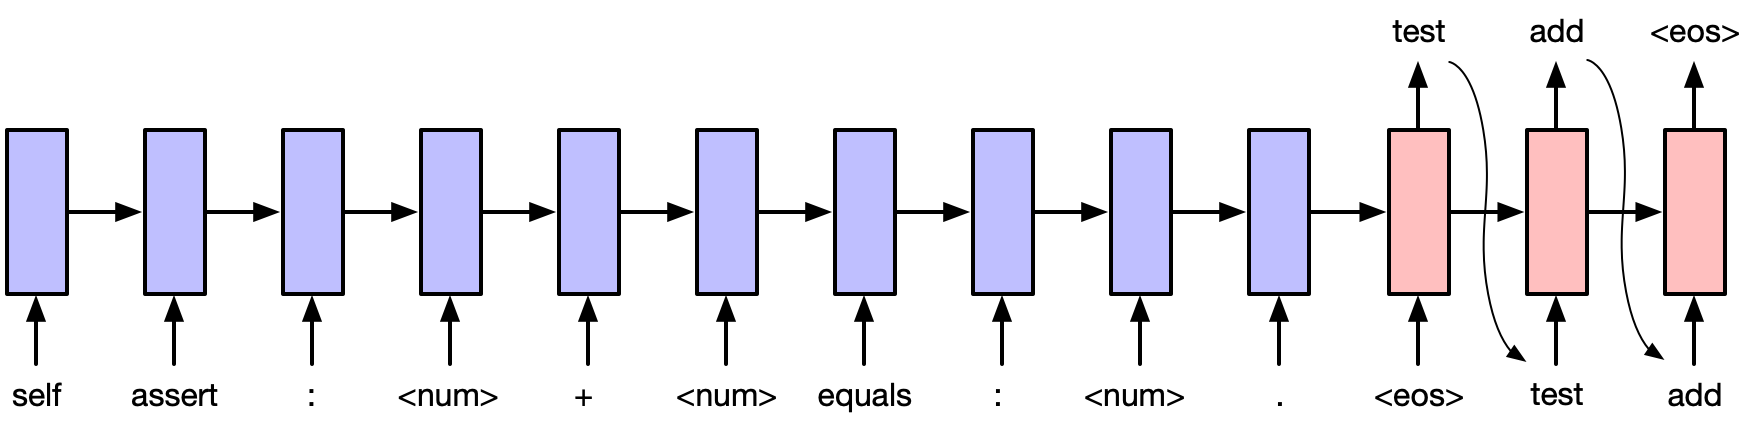
\includegraphics[width=\columnwidth]{seq2seq}
\end{figure}

Attention mechanism ensures that extent to which a certain token of the input sequence $x_k$ affects the output does not depend on its position $k$. This was especially important in our case. On average English, sentences have around 20 words. But the average number of source tokens in methods from our dataset exceeds 130. By using attention we can be sure that by the time the information from first tokens reaches the decoder, it will not be saturated. Regardless of its position in the input sequence, every token has the same chance to affect the decision and the only decoder decides to which tokens it wants to pay more attention.

We used GRU cells to avoid exploding and vanishing gradient and chose them over LSTM because they have fewer parameters to train and allow us to learn faster. Because of the big length of input sequences that we feed to our network we chose the hidden vector of size 256, which is larger than what is typically used for machine translation with the sequence to sequence networks.

\section{First look at the results}
\label{sec:TranslatingCode-Results}

In this section, we do a manual overview of the method names proposed by our model. Different approaches to the numeric evaluation of these results are discussed in Chapter \ref{chap:Evaluation}. All methods presented in this section are taken from the test set. The model has not seen any of them during training.

% , briefly discuss their validity and explore the attention to see the connection between certain source tokens and the generated names.

\begin{lstlisting}
"Real name:       test is comment
 Generated name:  test is comment"
self assert: self newNode isComment.
\end{lstlisting}

\begin{lstlisting}
"Real name:       color
 Generated name:  color"
r := aColor red.
g := aColor green.
b := aColor blue.
a := aColor alpha.
\end{lstlisting}

\begin{lstlisting}
"Real name:       accept with
 Generated name:  accept"
aVisitor
  visitDraggableInteractreion: self
  with: args.
\end{lstlisting}

\begin{lstlisting}
"Real name:       add package
 Generated name:  add package"
aPackage isPackage ifFalse: [^self].
self
  addElement: aPackage
  in: self packages.
\end{lstlisting}
%
% {\lstset{basicstyle=\footnotesize}
% \begin{table}[H]
%   \begin{tabular}{|L{7cm}|l|l|}
%     \hline
%     Source code &
%     Proposed name &
%     Real name \\
%     \hline
% \begin{lstlisting}
% self assert: self newNode isComment.
% \end{lstlisting} &
%     test is comment &
%     test is comment \\
%     \hline
% \begin{lstlisting}
% r := aColor red.
% g := aColor green.
% b := aColor blue.
% a := aColor alpha.
% \end{lstlisting} &
%     color &
%     color \\
%     \hline
% \begin{lstlisting}
% aVisitor
%   visitDraggableInteractreion: self
%   with: args.
% \end{lstlisting} &
%     accept &
%     accept with \\
%     \hline
% \begin{lstlisting}
% aPackage isPackage
%   ifFalse: [^self].
% self
%   addElement: aPackage
%   in: self packages.
% \end{lstlisting} &
%     add package &
%     add package \\
%     \hline
%   \end{tabular}
% \end{table}}

\chapter{Evaluation}
\label{chap:Evaluation}
\mtoc

In this chapter, we evaluate the method names generated by our model. We start by discussing the complexity of such an evaluation. Then we describe several metrics that we have selected for automatic evaluation, apply them to the generated names, and compare the scores of our model to several baseline models.

\section{Why is it hard to evaluate names?}
\label{sec:Evaluation-WhyHard}

While consistency of naming can be evaluated using simple heuristics that measure how much does a given name fit into the family of existing names, there is no objective way to tell how well does a given name represent certain concepts, usage, or implementation details. Human languages are complex and not formal. There can be many ways of describing the purpose of a method, class, or variable in 2-5 English words. And there can be many opinions on how comprehensive and informative a certain name is.

\subsection{Human evaluation}

Since our goal is to improve the readability of source code, the best way to evaluate the conciseness of identifier names would be asking a group of developers to evaluate them independently and then aggregating these results to produce a single score that would be most representative of human comprehension. The main drawback of human evaluation is its high cost in terms of human-hours and very low speed of evaluation. This means that we can only evaluate a reasonably small subset of methods using human experts and can only conduct this evaluation once or twice.

\subsection{Automatic evaluation}

Automatic metrics such as precision can be calculated quickly and do not require any additional expenses or involvement of human experts. The disadvantage of those metrics is the fact that they are very simplified approximate measures of goodness and informativeness of method names which nevertheless are very useful in practice.

Automatic metrics can only compare generated names to a set of reference names provided by humans that are considered to be a golden standard. More specifically, precision can measure the percentage of words in a generated method name that also appear in the real name of that method. When averaged over a big dataset of methods, precision can be very useful for comparing two different models. However, it can not be reliably used for evaluating a single name or interpreted as a standalone measure of model's performant because everything that is different from a reference name will be given a score of $0$. Automatic metrics are very simple measures that cannot recognize synonyms or different grammatical forms of words.

For example, if the real method name is \texttt{sumOfIntegers}, a reasonably good name such as \texttt{addAllIntegerNumbers} will be scored with 0 by all metrics discussed in the following section, because none of the words in those names match exactly. However, as we have seen in section \ref{sec:Naturalness-Vocabulary}, vocabulary used by programmers is very limited. Synonyms and different word forms are rather rare in practice, which means that in real-world scenarios automatic metrics can provide a pretty good approximation of the true model performance.

\section{Automatic evaluation}

As we said before, all metrics for automatic evaluation of method names are based on comparing the \textbf{generated name} to one or more \textbf{reference names} that are given by humans and considered the ground truth. Since all methods in our study were collected from real projects, each of them has exactly one name associated with it that was given by a programmer.

\subsection{Hypothesis for automatic evaluation}

As it was explained in Section \ref{sec:Evaluation-WhyHard}, automatic metrics are very simplified and imperfect. However, we can use them to compare different models based on the hypothesis that on average better model will generate more names similar to the real names of the methods.

\begin{quote}
Given a set of method bodies and a set of real method names, on average the names generated by a good model will be more similar to real names than the names from a bad model.
\end{quote}

It is important to keep this assumption in mind when looking at the results of the automatic evaluation and remember that it only holds when averaging multiple scores. On the level of individual observations, a method name with low precision score can be more relevant and informative than the name with a higher score.

\subsection{Selecting metrics}
\label{sec:Evaluation-Metrics}

In this section, we define the metrics that we have used for the automatic evaluation of method names generated by our model. We explain how each one of them works and provide examples of method names together with scores assigned to them by the metric in question. The method names in our examples were selected to demonstrate differences between those metrics:

\begin{description}
  \item [\texttt{testIsInteger}] \hfill \\
      --- exactly matches the reference name
  \item [\texttt{isIntegerTest}] \hfill \\
      --- has all the same words as the reference name but in different order
  \item [\texttt{testInteger}] \hfill \\
      --- has 2 out of 3 words of the reference name
  \item [\texttt{testIntegerNumber}] \hfill \\
      --- has 2 out of 3 words of the reference name and one additional word
  \item [\texttt{testIsIntegerNumber}] \hfill \\
      --- has all words of the reference name and one additional word
\end{description}

\paragraph{Exact match} --- percentage of generated method names that match reference names exactly (including the order of words). This metric was inspired by \cite{Alla16}.

\begin{table}[H]
\centering
\begin{tabular}{|l|r|}
  \hline
  testIsInteger & 1.00 \\
  \hline
  isIntegerTest & 0.00 \\
  \hline
  testInteger & 0.00 \\
  \hline
  testIsNumber & 0.00 \\
  \hline
  testIsIntegerNumber & 0.00 \\
  \hline
\end{tabular}
\caption{Exact match scores of names generated for a method with real name testIsInteger}
\end{table}

\paragraph{Precision} --- percentage of words in the generated name that appear in a reference name. It is calculated as a fraction of true positives ($\TP$\footnote{We use the following notation: $\TP$ - number of true positives, $\FP$ - number of false positives, $\TN$ - number of true negatives, $\FN$ - number of false negatives}) - number of words that appear both in reference and the generated name, by the total number of words in a generated name ($\TP + \FP$).

\[
\precision = \frac{\TP}{\TP + \FP}
\]

\begin{table}[H]
\centering
\begin{tabular}{|l|r|}
  \hline
  testIsInteger & 1.00 \\
  \hline
  isIntegerTest & 1.00 \\
  \hline
  testInteger & 1.00 \\
  \hline
  testIsNumber & 0.67 \\
  \hline
  testIsIntegerNumber & 0.75 \\
  \hline
\end{tabular}
\caption{Precision scores of names generated for a method with real name testIsInteger}
\end{table}

\paragraph{Recall} --- percentage of words in the reference name that appear in a generated name. It is calculated as a fraction of true positives ($\TP$) - the number of words that appear both in reference and the generated name, by the total number of words in a reference name ($\TP + \FN$).

\[
\recall = \frac{\TP}{\TP + \FN}
\]

\begin{table}[H]
\centering
\begin{tabular}{|l|r|}
  \hline
  testIsInteger & 1.00 \\
  \hline
  isIntegerTest & 1.00 \\
  \hline
  testInteger & 0.67 \\
  \hline
  testIsNumber & 0.67 \\
  \hline
  testIsIntegerNumber & 1.00 \\
  \hline
\end{tabular}
\caption{Recall scores of names generated for a method with real name testIsInteger}
\end{table}

\paragraph{F1} --- harmonic mean\footnote{Harmonic mean is more intuitive than the arithmetic mean when computing a mean of ratios} of precision and recall (\cite{Sasa07}).

\[
\fone = 2 \cdot \frac{\precision \cdot \recall}{\precision + \recall}
\]

\begin{table}[H]
\centering
\begin{tabular}{|l|r|}
  \hline
  testIsInteger & 1.00 \\
  \hline
  isIntegerTest & 1.00 \\
  \hline
  testInteger & 0.80 \\
  \hline
  testIsNumber & 0.67 \\
  \hline
  testIsIntegerNumber & 0.86 \\
  \hline
\end{tabular}
\caption{$\fone$ scores of names generated for a method with real name testIsInteger}
\end{table}

% \subsubsection{BLEU}
%
% Bilingual evaluation understudy (\bleu), introduced by \cite{Papi02}, is the most commonly used metric for automatically evaluating machine translation.

\subsection{Baseline models for comparison}
\label{sec:Evaluation-Baselines}

To evaluate the performance of our model using automatic metrics described in Section \ref{sec:Evaluation-Metrics} we compare them to several simple baseline models applied to the same dataset.

\subsubsection{Random model}

When evaluating machine learning models, it is always important to understand what would the values of all selected metrics be if the model did not learn anything but only made random choices. For example, in the problem of handwritten digit recognition on a well-balanced dataset\footnote{Take MNIST dataset for example: \url{http://yann.lecun.com/exdb/mnist/}} 10\% accuracy can be achieved by randomly selecting one of the 10 digits. If the trained model has significantly more than 10\% accuracy, we can say that it has recognized some patterns in the data and learned to use them.

Our random model makes assumption that all words in vocabulary are uniformly distributed (equally likely to appear at any position in a name of any method) and generates names for test set methods by selecting $K$ random words from the training set vocabulary (vocabulary from which the words are selected is the output vocabulary described in Section \ref{sec:TranslatingCode-EncodingTokens} that was constructed from method names in the training set). In our case, $K=3$ is the average number of tokens in the method names from our dataset. We do not use the test set vocabulary because it can have words that are not present in the training set. This simulates the real-world situation as we can not know in advance the complete vocabulary that people will use for naming new methods to which our model will be applied.

\subsubsection{TF-IDF model}

\textit{Term Frequency - Inverse Document Frequency} (TF-IDF) is a measure of word importance. It works by determining the relative frequency of a word in a specific method compared to the inverse proportion of that word over the entire corpus of source code. Intuitively, this calculation determines how relevant a given word is in a particular method (\cite{Ramo03}). Words that is rare in the entire source code corpus, but appears a lot in the code of a particular method must be strongly related to the concepts that describe the purpose of that method. Words that are common in all methods such as \texttt{self}, \texttt{if}, \texttt{true} receive low TF-IDF scores and are not selected into the method name.

Despite its simplicity and the fact that it generates method names using the source code vocabulary, TF-IDF algorithm achieves surprisingly good results in terms of automatic metrics described in Section \ref{sec:Evaluation-Metrics}. This is a simple and effective statistical technique that can be used as a good baseline to compare our model to.

TF-IDF score of a word $w$ in method $m$ that is part of a source code corpus $C$ is computed as a product of its \textit{term frequency} (TF) and \textit{inverse document frequency} (IDF).

\[ \tfidf(w, m, C) = \tf(w, m) \cdot \idf(w, C) \]

Where term frequency is defined as $f_{w,m}$ - number of times word $w$ appears in the source code of method $m$.

\[ \tf(w, m) = f_{w,m} \]

And inverse document frequency is the logarithm of $|C|$ - total number of words in source code corpus $C$ divided by $f_{w,C}$ - the number of methods in $C$ in which the word $w$ appears.

\[ \idf(w, C) = \log \frac{|C|}{f_{w,C}} \]

Multiplying term frequency of a word by its inverse document frequency we penalize words that frequently occur in the language (see Section \ref{sec:Naturalness-SpecializedVocabulary}) and select only those that are frequent in a given context\footnote{In Section \ref{sec:Conclusion-TFIDF} where we describe a potential direction of future work you can find an interesting example of how TF-IDF can be used to group packages by their conceptual similarity.}. The algorithm computes TF-IDF scores for every token in the source code of a method and selects $K=3$ words with the highest score into the name.


\subsection{Results of automatic evaluation}

In this section, we present the numeric results of the automatic evaluation and use it to compare the performance of our model to the selected baseline models described in Section \ref{sec:Evaluation-Baselines}.

In Section \ref{sec:TranslatingCode-TrainValidTest} we have talked about splitting our dataset into three subsets for training, validation, and testing. The small size of the validation set and the fact that automatic metrics described in Section \ref{sec:Evaluation-Metrics} can be computed very quickly allowed us to perform an evaluation of our model every 1000 iterations of its training. On Figure \ref{fig:ValidScores} you can see how the performance of the model measured by different metrics improves during training and how it surpasses the TF-IDF baseline applied to the same methods from the validation subset. The random model baseline cannot be seen on this graph because all its scores are very close to 0.

\begin{figure}[H]
    \centering
    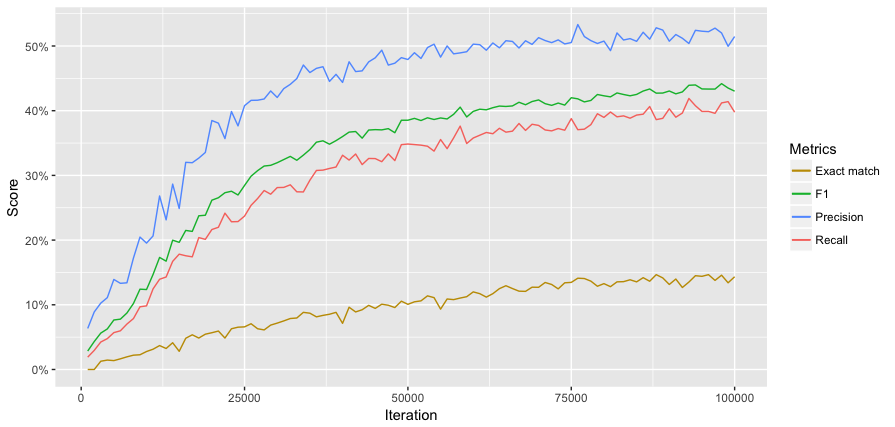
\includegraphics[width=\linewidth]{valid_scores}
  \caption{Evaluation of our model during training. Every 1000 iterations we applied the model to the validation set and measured all scores. Every score is compared to the corresponding value of the TF-IDF baseline (dashed lines)}
  \label{fig:ValidScores}
\end{figure}

Finally, we report the scores of our model together with baseline models measured on an independent test set which was never seen neither by model during training nor by us during model selection.

\begin{table}[H]
\centering
\begin{tabular}{|l|r|r|r|r|r|r|}
  \hline
  & Exact match & Precision & Recall & F1 \\
  \hline
  Our model & 13.82\% & 51.09\% & 38.92\% & 42.47\% \\
  \hline
  TF-IDF & 0.32\% & 28.61\% & 38.54\% & 30.95\% \\
  \hline
  Random model & 0\% & 0.07\% & 0.08\% & 0.07\% \\
  \hline
\end{tabular}
\caption{Results of automatic evaluation of method names generated by the selected models for methods from the test set}
\label{tab:Evaluation-TestResults}
\end{table}

In Table \ref{tab:Evaluation-TestResults} you can see the numeric scores of our model compared to selected baselines on the test set. First of all, notice that the random model has all scores close to 0. Both our model and TF-IDF perform significantly better, which proves that they indeed extract a lot of information from source code and successfully learn to generate method names. Our attention-based sequence to sequence deep neural network outperforms TF-IDF in terms of all metrics. By choosing parameters that maximize the likelihood of method names from our training set (see Section \ref{sec:TranslatingCode-Problem} and \ref{sec:Background-Likelihood}) our model guesses over 50\% of tokens from the previously unseen test set names.

Exact match is an interesting score because it demonstrates the ability of the model to not only to select frequent and relevant words but also put them in the correct order. Despite the fact that method name can be any combination of words from the vocabulary, which gives us really big space of possible names (and explains 0\% of exact match achieved by random model), our model guesses almost 14\% of names exactly. One can suspect that those are single word names. However, as you can see in Table \ref{tab:Evaluation-ExactMatches},  most of the exactly matched names have more than one word and some of them are novel names that have never appeared in the training set.

\begin{table}[H]
\centering
\begin{tabular}{|l|r|r|r|r|}
  \hline
  \textbf{Length} & \textbf{Unique names} & \textbf{\% of test set} & \textbf{Appear in train set} & \textbf{Novel names} \\
  \hline
  1 word & 249 & 6.63\% & 245 & 4 \\
  \hline
  2 words & 351 & 5.80\% & 301 & 50 \\
  \hline
  3 words & 108 & 1.09\% & 75 & 33 \\
  \hline
  4 words & 16 & 0.19\% & 11 & 5 \\
  \hline
  5 words & 10 & 0.09\% & 10 & 0 \\
  \hline
  6 words & 1 & 0.01\% & 1 & 0 \\
  \hline
  8 words & 1 & 0.01\% & 1 & 0 \\
  \hline
\end{tabular}
\caption{Distribution of names generated by our model that match real method names exactly over the length of the name (number of sub-token words). Columns of this table show the number of unique names in each group, what percent of all names from training set are in the group, how many of those names appeared in training set (but were paired with different source code), and how many names were never seen by the model before}
\label{tab:Evaluation-ExactMatches}
\end{table}

It is worth noting that despite its simplicity, TF-IDF performs reasonably well. Deep models are expensive both in terms of training and the complexity of deployment: big memory consumption by a trained model, high overhead when producing a single result. So in those cases when deep learning may be inapplicable, a simpler statistical model such as TF-IDF can be combined with other algorithms (for example, n-gram model for ordering words or hand-written heuristics) to produce very good results.

% \section{Human evaluation}
%
% \subsection{Design of questionnaire}
%
% \subsection{Results of evaluation}

\chapter{Conclusion}
\label{chap:Conclusion}
\mtoc

We conclude this work by summarizing our discoveries, discussing their importance and talking about the potential directions of future work.

\section{What we discovered}

In this work we have answered the two most important questions that were stated in Section \ref{sec:Introduction-Problem}:

\begin{RQ}
  \item \textbf{Is source code of Pharo natural enough to allow us to use its regularities in machine learning models?} By measuring statistical properties of our dataset in Section \ref{sec:Naturalness-CrossEntropy} and comparing the source code of two programming languages, Pharo and Java, and different corpora of English language we have shown that programming languages have a much smaller vocabulary and introduce more domain-specific words than English texts. The source code is also highly repetitive. This suggests that applying predictive models to it can be even more effective than to natural text, and after proper preprocessing of code such applications on Pharo should not be less effective then successful experiments that were reported on Java.

  \item \textbf{Does source code of a method contain enough semantic information to generate a name that would express the purpose of that method?} Although, as we have mentioned in Section \ref{sec:Introduction-Problem} programmers do not choose names for methods base on their implementation details, our model was able to generate method names with precision over 50\% when compared to real names and 14\% of generated names matching true names exactly. We also report F1 score of almost 32\% using TF-IDF model which generates names by selecting important words from source code. The high performance of both models that deduce method names exclusively from source code can be explained by high repetitiveness of code, mentioned in section \ref{sec:Naturalness-Repetitive} and the semantic information carried by identifier names (local variable names, method calls, class names).
\end{RQ}

\section{Directions of future work}

\subsection{Additional features}

As we have mentioned in  Section \ref{sec:Introduction-Problem}, good method names describe how they should be used (for example, sorting algorithms may have different implementation, but they are all used for sorting and called \texttt{sort}) and what actions they model (for example, the same method which moves an object from point A to point B can be called \texttt{drive} if the receiver is a \texttt{Car} or \texttt{fly} if its an \texttt{Airplane}). This suggests that in practical applications the information about class hierarchy of the receiver and the usage context such as slices of code surrounding method calls can be used as additional features for modelling method names.

\subsection{Grouping packages by conceptual similarity}
\label{sec:Conclusion-TFIDF}

The effective application of TF-IDF to extracting keywords from source code demonstrated in Chapter \ref{chap:Evaluation} suggests that this simple statistical technique can be used for concept mining in software packages and classes. A list of $N$ most relevant keywords in the source code of a package will be semantically related to the concepts modelled by that package.

\begin{table}[H]
\centering
\begin{tabular}{|l|l|}
  \hline
  \textbf{Package} & \textbf{Top 5 keywords} \\
  \hline
  Roassal2 & shape, view, color, es, elements \\
  Athens-Text & color, font, nn, current, fnt \\
  Athens-Examples & canvas, paint, path, @, draw \\
  Athens-Morphic & canvas, transform, zoom, rect, rectangle \\
  Morphic-Core & menu, morph, bounds, event, world \\
  Morphic-Widgets-Basic & style, color, state, button, morph \\
  Morphic-Widgets-FastTable & row, indexes, index, scroll, rows \\
  Math-Matrix & rows, n, matrix, row, matrices \\
  Math-Core & n, radix, product, precision, vector \\
  Math-Polynomials & coefficients, degree, n, remainder, quotient \\
  Calypso-Browser & browser, navigation, items, query, tool \\
  \hline
\end{tabular}
\caption{Keywords extracted from Pharo packages using TF-IDf scores}
\end{table}

Given that $V$ is the vocabulary of tokens used in source code, for every package TF-IDF will provide a numeric vector of relevance scores for every word in $V$. We can assume that packages that model similar concepts will be assigned with similar TF-IDF vectors. And by measuring the distance between those vectors (for example, cosine similarity), we can cluster software packages into groups by their conceptual similarity.

\begin{table}[H]
\centering
\begin{tabular}{|l|p{9cm}|}
  \hline
  \textbf{Package} & \textbf{Top 5 similar packages} \\
  \hline
  Roassal2 & Trachel, DataFrame-Tools, Roassal2GT, Geometry, Morphic-Base \\
  \hline
  Geometry & Graphics-Tests, SortFunctions-Tests, Balloon-Tests, Roassal2, Trachel\\
  \hline
  DataFrame-Core & DataFrame-Core-Tests, DataFrame-Tools-Tests, GT-Spotter-EventRecorder, Tabular, Math-Tests-Matrix \\
  \hline
\end{tabular}
\caption{Keywords extracted from Pharo packages using TF-IDf scores}
\end{table}

This would allow us to build tools for improving the consistency and conciseness on source code not on package level or entire corpus level, but on the level of groups of conceptually similar packages.


%----------------------------------------------------------------------------------------
%	THESIS CONTENT - APPENDICES
%----------------------------------------------------------------------------------------

\appendix % Cue to tell LaTeX that the following "chapters" are Appendices

% Include the appendices of the thesis as separate files from the Appendices folder
% Uncomment the lines as you write the Appendices

\chapter{Theoretical background}
\label{chap:Background}
\mtoc

In this chapter, we provide a brief overview of the main concepts of natural language processing required to understand the rest of this work.

\section{Language models}
\label{sec:Background-LanguageModels}

Language models are probabilistic models that predict the next word in a sequence. They also assign probabilities all possible sentences and sequences of words constructed from the words of a given language (\cite{Jura09}).

We train language models on large corpora of text written in a given language. For example, by counting occurrences and co-occurrences of words. A language model trained on a big enough English corpora should assign a higher probability to the first sentence and consider the second one very unlikely.

\begin{enumerate}
\item Today is a rainy day here in Paris.
\item Nice not such but inside in after.
\end{enumerate}

Finding the probability distribution of words is an important part of many NLP problems, such as spellchecking, error correction, or machine translation. As we will see in Section \ref{sec:Background-seq2seq}, state of the art recurrent neural network used for machine translation are also very advanced language models.

\section{Entropy and cross-entropy}

The amount of information produced when one message is chosen from the set of possible messages can be measured as

\[ I(x) = -log_2 P(x) \]

It was \cite{Shan48} who proposed to use the logarithm with base 2 and call the units of information bits (or binary digits). We can also use natural logarithm but then the units of measurement will be called nats.

\subsection{Entropy}

In information theory, a random variable is treated as a source of information. The entropy of variable X is the expectation of the amount of information in the outcome (\cite{Mack03}).

\[ H(X) = \mathbb{E}\big[ I(x) \big] = - \mathbb{E}\big[ log P(x) \big] \]

In the context of languages, we only consider discrete random variables over the finite alphabet.

\[ H(X) = - \sum_{i=1}^N P(x_i) log P(x_i) \]

Entropy is considered the measure of uncertainty of variable X.

\subsection{Kullback-Leibler divergence}
\label{sec:Background-KL}

The difference between two probability distributions is measured with a Kullback-Leibler (KL) divergence:

\[ D_{KL}(P||Q) = \mathbb{E}\bigg[ \log \frac{P(x_i)}{Q(x_i)} \bigg] = \mathbb{E}\big[ \log P(x_i) - \log Q(x_i) \big] \]

For the case of discrete variables

\[ D_{KL}(P||Q) = \sum_{i=1}^N P(x_i) \log \frac{P(x_i)}{Q(x_i)} \]

\subsection{Cross-entropy}

Cross-entropy is the average number of bits needed to encode data from the source with distribution P when we use model Q to define our codebook (\cite{Murp13}).

\[ H(P, Q) = - \sum_{i=1}^N P(x_i) log Q(x_i) \]

It can be expressed as a sum of entropy and KL divergence

\begin{equation}
    H(P, Q) = H(P) + D_{KL}(P||Q)
    \label{eq:KL-Entropy}
\end{equation}

The lower bound of cross-entropy means that even if we find the perfect model which matches the true distribution of data, cross-entropy will not be lower than the entropy of this dataset.

\subsection{Why do we minimize the cross-entropy?}
\label{sec:Background-Likelihood}

Many problems in machine learning can be viewed as function estimation: we are trying to predict a variable $y$ given an input vector $x$ (\cite{Good16}). We assume that there is a true function $f(x)$ that describes relationship between $x$ and $y$. All other factors that influence $y$ are considered to be noise $\epsilon$ (in real world nothing is really influenced by a single factor; be it a coin toss or a roll of dice, outcome of any process is affected by more factors than we could possibly measure, however, the effect of most factors is so insignificant that they can be ignored).

\[ y = f(x) + \epsilon \]

We want to find function $\hat{f}$ (model, estimate) which is as close as possible to the "true" function $f$. When we say that we are training a machine learning model, we mean that we choose a model, which is a parametrised function $\hat{f}(x;\theta)$ and iteratively move it closer to the "true" function $f$ by changing the parameter $\theta$.

In probabilistic interpretation the process that we are trying to model, or function $f$, is the "true" probability distribution $P_{data}(x, y)$ that generates a set of $(x, y)$ points. We observe this process by collecting the training data $D =\{(x^{(i)}, y^{(i)})|i=1,2,\dots\}$ and try to model it with a parametric family of distribution $P_{model}(x, y; \theta)$ (function $\hat{f}$) by finding such parameter $\theta^{*}$ which minimizes the difference between those two distributions. As we mentioned in Section \ref{sec:Background-KL}, the difference between two distributions is measured with a Kullback-Leibler divergence.

\[ \theta^{*} = \argmin_{\theta} D_{KL}(P_{data}||P_{model}) \]

And based on Equation \ref{eq:KL-Entropy}, this is the same as minimizing the difference between the cross-entropy of our model applied to the dataset $H(P_{data}, P_{model})$ and the entropy of this dataset $H(P_{data})$

\[ \theta^{*} = \argmin_{\theta} \bigg[H(P_{data}, P_{model}) - H(P_{data})\bigg] \]

Since $P_{data}$ does not depend on $\theta$ and can not be controlled by us, this boils down to minimizing the cross-entropy:

\[ \theta^{*} = \argmin_{\theta} H(P_{data}, P_{model}) \]

Now we will show that this is the same as maximizing the likelihood of the dataset $D$ assigned to it by our model $P_{model}$. The likelihood is the measure of how likely is our model to produce this dataset. We assume that by choosing the model which has highest likelihood of generating dataset $D$ we will get a model that behaves like the true process in other situations (this really depends on how representative is $D$ of the entire distribution $P_{model}$ and whether we are able to generalize and not overfit - simply memorize - the training data $D$). The likelihood is expressed as the probability that our model $P_{model}$ assigns to the dataset $D$. So we want to find parameter $\theta^{*}$ which maximizes this probability:

\[ \theta^{*} = \argmax_{\theta} P_{model}(D;\theta) \]

We make an assumption that all points in $D$ are independent of each other, which allows us to express the probability of generating dataset $D$ into the product of probabilities of generating each one of its points. If $m = |D|$ is the size of our dataset,

\[ P_{model}(D;\theta) = \prod_{i=1}^m P_{model}(x^{(i)}, y^{(i)};\theta) \]

Which means that

\[ \theta^{*} = \argmax_{\theta} \prod_{i=1}^m P_{model}(x^{(i)}, y^{(i)};\theta) \]

To simplify this task, we can use the property of logarithms which turns product into a sum, and maximize the logarithm of expression on the right. Indeed the same parameter $\theta^{*}$ which maximizes the logarithm of an expession, will also maximize that expression. Therefore,

 \[ \theta^{*} = \argmax_{\theta} \log \prod_{i=1}^m P_{model}(x^{(i)}, y^{(i)};\theta) \]
 \[ = \sum_{i=1}^m \log P_{model}(x^{(i)}, y^{(i)};\theta) \]

 The logarithm of a likelihood (right-hand side expression) is called log-likelihood. In the same way, we can multiply this expression by any constant without changing the maximization parameter. Let's normalize it over the size of our dataset

 \[ \theta^{*} = \argmax_{\theta} \frac{1}{m}\sum_{i=1}^m \log P_{model}(x^{(i)}, y^{(i)};\theta) \]

 This, in fact is the expectation of log-pobability of random point with respect to the probability distribution $P_{data}$:

 \[ \theta^{*} = \argmax_{\theta} \mathbb{E}_{(x,y) \sim P_{data}} \bigg[\log P_{model}(x, y;\theta)\bigg] \]

 Which is the same as minimizing the negative expectation, or cross-entropy:

 \[ \theta^{*} = \argmin_{\theta} - \mathbb{E}_{(x,y) \sim P_{data}} \bigg[\log P_{model}(x, y;\theta)\bigg] \]

  \[ = \argmin_{\theta} H(P_{data}, P_{model}) \]

This explains why we train machine learning models by minimizing cross-entropy and why it is the same as maximizing the likelihood. Every cost function is, in fact, the cross-entropy of empirical distribution $P_{data}$ and some the distribution that we choose for our model. For example, mean squared error (MSE) is cross-entropy of $P_{data}$ and the normal distribution.

\section{Recurrent neural networks}
\label{sec:Background-RNN}

A big limitation of feedforward neural networks is the fact that they require a fixed-size input and always produce a fixed-size output. For example, a network that has 2 neurons in the input layer and 1 neuron in the output layer can only accept vectors of size 2 and return vectors of size 1.

Some problems, however, require processing of sequential data. This includes time series forecasting, music composition, and many tasks of natural language processing, such as machine translation, text summarization, question answering, sentiment analysis, speech recognition, text-to-speech and speech-to-text translation etc. The input of these problems is a sequence of variable length.

\textbf{Recurrent neural networks} (RNN) are a special kind of neural networks that have cyclical connections. At every step, such networks receive a fixed-size input (for example, one word) and the information from the previous step, transmitted through the cyclical connection. This creates memory inside a network which allows it to operate on sequences of input values.

\begin{figure}[H]
    \label{fig:rnn}
    \centering
    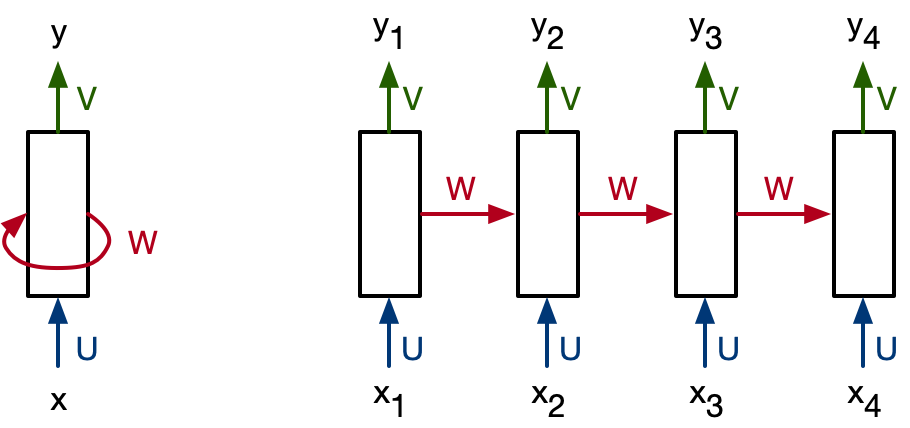
\includegraphics[height=4cm]{rnn}
\end{figure}

\subsection{Sequence to sequence networks}
\label{sec:Background-seq2seq}

On each step, recurrent neural network receives an input value, produces the output value, and passes its internal state onto the next step. From this follows:

\begin{enumerate}
    \item Sequence of $N$ inputs will produce a sequence of $N$ outputs.
    \item Every output $y_k$ is only affected by the current input $x_k$ and all the previous inputs $x_1, \dots x_{k-1}$ but not the next inputs $x_{k+1}, \dots, x_N$
\end{enumerate}

This is useful for problems like predicting next element in a sequence, but other tasks may require input and output sequences to be of different sizes and the output to be equally affected by all elements of input.

Consider a question answering system. A neural network receives a sequence of words in a question: \textit{"At what temperature does water boil?"} and produces the answer: \textit{"Water boils at 100 degrees."}. Such answer cannot be produced by a classical RNN because the length of a question exceeds the length of the answer and it is impossible to produce the beginning of the answer \textit{"Water boils ..."} until we have seen the end of the question \textit{"... does water boil"}.

This can be done by a special combination of two recurrent neural network called \textbf{sequence to sequence} or \textbf{encoder-decoder neural network} neural networks introduced by \cite{Suts14}.

\paragraph{Encoder} is a recurrent neural network which accepts the sequence of input values. The output of encoder is ignored and the state vector received on the last step encodes the input sequence (sometimes called "thought vector").

\paragraph{Decoder} is another recurrent neural network which receives its own output from the previous step as input on the current step and generates the output sequence. On the first step, a decoder receives the encoded sequence provided by the encoder as its internal state.

Putting encoder and decoder together we receive a neural network which first reads the whole input sequence of size $N$ and only then produces the output sequence of size $M$, making it possible that $N \neq M$.

Sequence to sequence networks are in fact language models that learn the probability distribution of the output sequences conditioned by the input sequences. They are widely used in machine translation, question answering, text summarization, and many other similar applications.

\subsection{LSTM and GRU cells}
\label{sec:Background-LSTMandGRU}

The major problem with recurrent neural networks is vanishing or exploding gradient. As the network is trained on a sequence of input, we use the algorithm called "backpropagation through time" which propagates an error back through the cyclical connection reversing the path made by the input sequence. This process is similar to backpropagating an error through the deep feedforward network with as many layers as the length of the input sequence. The only difference is that the weight matrix on each layer is now the same matrix corresponding to the cyclical connection. This leads to the problem described by \cite{Hoch01}: backpropagated error signals exponentially depend on the magnitude of weights. They tend to either explode if weights are above 1 or vanish if they are below.

As a solution to this problem \cite{Hoch97} introduced a novel method called \textbf{Long short-term memory (LSTM)} - memory cells with internal architecture that allows bridging very long time lags and does not suffer from exploding or vanishing gradient.

\cite{Cho14} proposed a simplified version of memory cells called \textbf{Gated recurrent unit (GRU)} which achieve similar performance to LSTM cells but have fewer parameters.


%----------------------------------------------------------------------------------------
%	BIBLIOGRAPHY
%----------------------------------------------------------------------------------------

% \printbibliography[heading=bibintoc]
\bibliographystyle{apalike}
\bibliography{others}

%----------------------------------------------------------------------------------------

\end{document}
